\documentclass{article}
\usepackage{float}
\usepackage{multirow}
\usepackage{booktabs} % For better tables
\usepackage{array} % For more control over table columns
\usepackage[T1]{fontenc}

%%%%%%%%%%%%%%%%%%%%%%%%%%%%%%%%%%%%%%%%%
% Lachaise Assignment
% Structure Specification File
% Version 1.0 (26/6/2018)
%
% This template originates from:
% http://www.LaTeXTemplates.com
%
% Authors:
% Marion Lachaise & François Févotte
% Vel (vel@LaTeXTemplates.com)
%
% License:
% CC BY-NC-SA 3.0 (http://creativecommons.org/licenses/by-nc-sa/3.0/)
% 
%%%%%%%%%%%%%%%%%%%%%%%%%%%%%%%%%%%%%%%%%

%----------------------------------------------------------------------------------------
%	PACKAGES AND OTHER DOCUMENT CONFIGURATIONS
%----------------------------------------------------------------------------------------

\usepackage{amsmath,amsfonts,stmaryrd,amssymb} % Math packages

\usepackage{enumerate} % Custom item numbers for enumerations

\usepackage[ruled]{algorithm2e} % Algorithms

\usepackage[framemethod=tikz]{mdframed} % Allows defining custom boxed/framed environments

\usepackage{listings} % File listings, with syntax highlighting
\lstset{
	basicstyle=\ttfamily, % Typeset listings in monospace font
}

\usepackage{subfigure}

%----------------------------------------------------------------------------------------
%	DOCUMENT MARGINS
%----------------------------------------------------------------------------------------

\usepackage{geometry} % Required for adjusting page dimensions and margins

\usepackage{setspace}

\onehalfspacing

\geometry{
	paper=a4paper, % Paper size, change to letterpaper for US letter size
	top=3cm, % Top margin
	bottom=3.5cm, % Bottom margin
	left=3cm, % Left margin
	right=3cm, % Right margin
	headheight=14pt, % Header height
	footskip=1.5cm, % Space from the bottom margin to the baseline of the footer
	headsep=1.2cm, % Space from the top margin to the baseline of the header
	%showframe, % Uncomment to show how the type block is set on the page
}

%----------------------------------------------------------------------------------------
%	FONTS
%----------------------------------------------------------------------------------------

\usepackage[utf8]{inputenc} % Required for inputting international characters
\usepackage[T1]{fontenc} % Output font encoding for international characters

\usepackage{XCharter} % Use the XCharter fonts

%----------------------------------------------------------------------------------------
%	COMMAND LINE ENVIRONMENT
%----------------------------------------------------------------------------------------

% Usage:
% \begin{commandline}
%	\begin{verbatim}
%		$ ls
%		
%		Applications	Desktop	...
%	\end{verbatim}
% \end{commandline}

\mdfdefinestyle{commandline}{
	leftmargin=10pt,
	rightmargin=10pt,
	innerleftmargin=15pt,
	middlelinecolor=black!50!white,
	middlelinewidth=2pt,
	frametitlerule=false,
	backgroundcolor=black!5!white,
	frametitle={Command Line},
	frametitlefont={\normalfont\sffamily\color{white}\hspace{-1em}},
	frametitlebackgroundcolor=black!50!white,
	nobreak,
}

% Define a custom environment for command-line snapshots
\newenvironment{commandline}{
	\medskip
	\begin{mdframed}[style=commandline]
}{
	\end{mdframed}
	\medskip
}

%----------------------------------------------------------------------------------------
%	FILE CONTENTS ENVIRONMENT
%----------------------------------------------------------------------------------------

% Usage:
% \begin{file}[optional filename, defaults to "File"]
%	File contents, for example, with a listings environment
% \end{file}

\mdfdefinestyle{file}{
	innertopmargin=1.6\baselineskip,
	innerbottommargin=0.8\baselineskip,
	topline=false, bottomline=false,
	leftline=false, rightline=false,
	leftmargin=2cm,
	rightmargin=2cm,
	singleextra={%
		\draw[fill=black!10!white](P)++(0,-1.2em)rectangle(P-|O);
		\node[anchor=north west]
		at(P-|O){\ttfamily\mdfilename};
		%
		\def\l{3em}
		\draw(O-|P)++(-\l,0)--++(\l,\l)--(P)--(P-|O)--(O)--cycle;
		\draw(O-|P)++(-\l,0)--++(0,\l)--++(\l,0);
	},
	nobreak,
}

% Define a custom environment for file contents
\newenvironment{file}[1][File]{ % Set the default filename to "File"
	\medskip
	\newcommand{\mdfilename}{#1}
	\begin{mdframed}[style=file]
}{
	\end{mdframed}
	\medskip
}

%----------------------------------------------------------------------------------------
%	NUMBERED QUESTIONS ENVIRONMENT
%----------------------------------------------------------------------------------------

% Usage:
% \begin{question}[optional title]
%	Question contents
% \end{question}

\mdfdefinestyle{question}{
	innertopmargin=1.2\baselineskip,
	innerbottommargin=0.8\baselineskip,
	roundcorner=5pt,
	nobreak,
	singleextra={%
		\draw(P-|O)node[xshift=1em,anchor=west,fill=white,draw,rounded corners=5pt]{%
		Question \theQuestion\questionTitle};
	},
}

\newcounter{Question} % Stores the current question number that gets iterated with each new question

% Define a custom environment for numbered questions
\newenvironment{question}[1][\unskip]{
	\bigskip
	\stepcounter{Question}
	\newcommand{\questionTitle}{~#1}
	\begin{mdframed}[style=question]
}{
	\end{mdframed}
	\medskip
}

%----------------------------------------------------------------------------------------
%	WARNING TEXT ENVIRONMENT
%----------------------------------------------------------------------------------------

% Usage:
% \begin{warn}[optional title, defaults to "Warning:"]
%	Contents
% \end{warn}

\mdfdefinestyle{warning}{
	topline=false, bottomline=false,
	leftline=false, rightline=false,
	nobreak,
	singleextra={%
		\draw(P-|O)++(-0.5em,0)node(tmp1){};
		\draw(P-|O)++(0.5em,0)node(tmp2){};
		\fill[black,rotate around={45:(P-|O)}](tmp1)rectangle(tmp2);
		\node at(P-|O){\color{white}\scriptsize\bf !};
		\draw[very thick](P-|O)++(0,-1em)--(O);%--(O-|P);
	}
}

% Define a custom environment for warning text
\newenvironment{warn}[1][Warning:]{ % Set the default warning to "Warning:"
	\medskip
	\begin{mdframed}[style=warning]
		\noindent{\textbf{#1}}
}{
	\end{mdframed}
}

%----------------------------------------------------------------------------------------
%	INFORMATION ENVIRONMENT
%----------------------------------------------------------------------------------------

% Usage:
% \begin{info}[optional title, defaults to "Info:"]
% 	contents
% 	\end{info}

\mdfdefinestyle{info}{%
	topline=false, bottomline=false,
	leftline=false, rightline=false,
	nobreak,
	singleextra={%
		\fill[black](P-|O)circle[radius=0.4em];
		\node at(P-|O){\color{white}\scriptsize\bf i};
		\draw[very thick](P-|O)++(0,-0.8em)--(O);%--(O-|P);
	}
}

% Define a custom environment for information
\newenvironment{info}[1][Info:]{ % Set the default title to "Info:"
	\medskip
	\begin{mdframed}[style=info]
		\noindent{\textbf{#1}}
}{
	\end{mdframed}
}

\usepackage{todonotes}

\nocite{*}
\usepackage{amsthm}

\theoremstyle{definition}
\newtheorem{theorem}{Theorem}[section]
\newtheorem{proposition}{Proposition}[section]
\newtheorem{definition}{Definition}[section]
\newtheorem{exercise}{Exercise}[section]
\newtheorem{subexercise}{}[exercise]


\newtoks\firstname
\newtoks\lastname
\newtoks\period
\newtoks\master
\newtoks\teacher
\newtoks\place
\newtoks\location

\makeatletter
\def\@maketitle{
\begin{titlepage}
    \centering
    
\includegraphics[width=0.15\textwidth]{logo-enpc}\par\vspace{1cm}
    {\scshape\LARGE École des Ponts ParisTech \par}
    \vspace{3cm}
    {\huge\bfseries \@title \par}
    \medskip
    {\Large\itshape \the\firstname~\the\lastname \par}
    \medskip
    {\large \@date \par}
    \vspace{1cm}
    {\Large Enseignant : \itshape \the\teacher \par}
\end{titlepage}
}
\makeatother


\usepackage{titlesec}
\usepackage{hyperref}

\titleclass{\subsubsubsection}{straight}[\subsection]

\newcounter{subsubsubsection}[subsubsection]
\renewcommand\thesubsubsubsection{\thesubsubsection.\arabic{subsubsubsection}}
\renewcommand\theparagraph{\thesubsubsubsection.\arabic{paragraph}} % optional; useful if paragraphs are to be numbered

\titleformat{\subsubsubsection}
  {\normalfont\normalsize\bfseries}{\thesubsubsubsection}{1em}{}
\titlespacing*{\subsubsubsection}
{0pt}{3.25ex plus 1ex minus .2ex}{1.5ex plus .2ex}

\makeatletter
\renewcommand\paragraph{\@startsection{paragraph}{5}{\z@}%
  {3.25ex \@plus1ex \@minus.2ex}%
  {-1em}%
  {\normalfont\normalsize\bfseries}}
\renewcommand\subparagraph{\@startsection{subparagraph}{6}{\parindent}%
  {3.25ex \@plus1ex \@minus .2ex}%
  {-1em}%
  {\normalfont\normalsize\bfseries}}
\def\toclevel@subsubsubsection{4}
\def\toclevel@paragraph{5}
\def\toclevel@paragraph{6}
\def\l@subsubsubsection{\@dottedtocline{4}{7em}{4em}}
\def\l@paragraph{\@dottedtocline{5}{10em}{5em}}
\def\l@subparagraph{\@dottedtocline{6}{14em}{6em}}
\makeatother

\setcounter{secnumdepth}{4}
\setcounter{tocdepth}{4} 

\title{PAMS's project} % Title of the assignment

\author{Alfonso Mateos Vicente\\ \texttt{alfonso.mateos-vicente@eleves.enpc.fr}} % Author name and email address

\date{École des Ponts ParisTech} % University, school and/or department name(s) and a date

\firstname{Alfonso}
\lastname{Mateos Vicente}
\teacher{Noé Blassel}
\master{Mme. Jane Doe}
\title{PAM's project}
\date{\today}

%-----------------------------------------------------------------------------


\begin{document}

\begin{titlepage}
    \newgeometry{left=3cm, right=3cm, top=2cm, bottom=2cm}
    \begin{center}
        \vspace*{1cm}
        
        \Huge
        \textbf{Simulation of Random Variables, Hamiltonian Dynamics, and Sampling via Markov Chains}
        
        \vspace{1.5cm}

        \Large
        \textbf{Author:} \\
        \vspace{0.25cm}
        \LARGE
        Alfonso Mateos Vicente \\
        \vspace{0.5cm}
        \Large
        \textbf{Tutor:} \\
        \vspace{0.25cm}
        \LARGE
        Noé Blassel

        \vfill
        
        
\includegraphics[width=0.2\textwidth]{./logo-enpc.eps}
        
        \vspace{1cm}
        
        \normalsize
        Ingénierie Mathématique et Informatique \\
        École des Ponts ParisTech \\
        France \\
        September 01, 2023
    \end{center}
    \restoregeometry
\end{titlepage}


\newpage
\tableofcontents
\newpage

\section*{Abstract}

This paper presents a comprehensive examination of simulation techniques in the realms of random variables, Hamiltonian dynamics, and Markov chain sampling. The initial section is devoted to the simulation of random variables, leveraging the Inverse Cumulative Distribution Function (CDF) method and Rejection Sampling method. Empirical validations of the Law of Large Numbers and the Central Limit Theorem are conducted to ascertain the efficacy of these methods. We also explore various variance reduction techniques, including control variates, importance sampling, stratified sampling, and antithetic variates, culminating in a detailed comparative analysis.

The subsequent section shifts focus to Hamiltonian dynamics, beginning with an introduction to the core principles, followed by an exploration of symplectic schemes. This includes analytical solutions, the Euler method, and a critical examination of the failure of standard methods. The development of Symplectic Schemes, particularly the Symplectic Euler and Stormer-Verlet methods, is presented with a comprehensive linear stability analysis. The application of these methods is illustrated through the simulation of the Solar System's gravitational dynamics, extending to experiments involving the N-Body Problem and the Symplectic Euler Method.

The paper culminates with a section on Sampling via Markov Chains. This section explores the application of Euler-Moruyama schemes to 2D potentials, delve into the intricacies of Langevin dynamics and splitting schemes, and present the final implementation in a full 2D molecular system. This aims to deepen the understanding of Markov chain sampling techniques and their practical applications in complex systems.

\newpage

\section{Simulation of Random Variables}
\label{sec:simulation_of_random_variables}

This section explores the simulation of random variables, a cornerstone in statistical and dynamical system studies. In Section 1.1, we introduce the Inverse CDF method (\ref{sec:inverse_cdf}), providing a foundational overview of its mechanics and application in simulating random variables.

Progressing to Section 1.2 (\ref{sec:rejection_sampling}), the manuscript transitions to the Rejection Sampling method. This section is further divided to enhance clarity and depth: Section 1.2.1 (\ref{sec:enveloping_distribution}) delves into the selection of the appropriate enveloping distribution, and Section 1.2.2 (\ref{sec:results_rejection_sampling}) presents the outcomes and insights from applying this method.

The narrative continues in Section 1.3 (\ref{sec:lln}), where the empirical validation of the Law of Large Numbers is discussed, and in Section 1.4 (\ref{sec:clt}), focusing on the Central Limit Theorem. These sections underscore the practical validation and implications of these pivotal statistical laws in simulation scenarios.

Concluding this section, a detailed examination of various variance reduction techniques is presented in Section 1.5 (\ref{sec:variance_reduction}). Starting with fundamental concepts in Section 1.5.1 (\ref{sec:variance_reduction_preliminaries}), it then explores control variates (Section 1.5.2, \ref{sec:control_variates}), importance sampling (Section 1.5.3, \ref{sec:importance_sampling}), stratified sampling (Section 1.5.4, \ref{sec:stratified_sampling}), and antithetic variates (Section 1.5.5, \ref{sec:antithetic_variates}), culminating in a comparative review in Section 1.5.6 (\ref{sec:comparative_review}). This part of the manuscript synthesizes and compares these techniques, highlighting their role in enhancing the accuracy and efficiency of simulation processes.

\subsection{Inverse CDF method}
\label{sec:inverse_cdf}

Inverse CDF method is a basic method to generate pseudo-random numbers from any probability distribution given its cumulative distribution function. First of all, let's introduce the following statement extracted from \cite{wikitInverseTransformSampling}:

\begin{theorem}[Inverse Transform Sampling]
	For any random variable $X \in \mathbb{R}$, the random variable $F_X^{-1}(U)$ has the same distribution as $X$, where $F_X^{-1}$ is the generalized inverse of the cumulative distribution function $F_X$ of $X$ and $U$ is uniform on $[0,1]$.

	For continuous random variables, the inverse probability integral transform is indeed the inverse of the probability integral transform, which states that for a continuous random variable $X$ with cumulative distribution function $F_X$, the random variable $U = F_X(X)$ is uniform on $[0,1]$.
\end{theorem}

Knowing this, the idea is to generate a uniform random variable \(U\) and then apply the inverse of the cumulative distribution function \(F^{-1}\) to obtain a random variable with the desired distribution. The Algorithm~\ref{alg:fastTwoSum} is as follows:

\begin{center}
	\begin{minipage}{0.7\linewidth} % Adjust the minipage width to accomodate for the length of algorithm lines
		\begin{algorithm}[H]
			1. Generate a set of random numbers \(U \sim \mathcal{U}(0,1)\) \;
			2. Find the inverse of the cumulative distribution function \(F^{-1}\) \;
			3. Apply the inverse to the set of random numbers \(X = F^{-1}(U)\) \;
			\caption{Inverse CDF mehtod} % Algorithm name
			\label{alg:fastTwoSum}   % optional label to refer to
		\end{algorithm}
	\end{minipage}
\end{center}

Let's see this with some examples. Using the exponential distribution, we know its probability density function is \(f(x) = \lambda e^{-\lambda x}\).  Also, we alredy know its cumulative distribution function which is \(F(x) = 1 - e^{-\lambda x}\). Then, the inverse of the cumulative distribution function is:

\begin{equation}\label{eq:inversecdf} F^{-1}(x)  = -\frac{1}{\lambda} \ln(1-x) \end{equation}

So, we can generate a set of random numbers \(U \sim \mathcal{U}(0,1)\) and apply the inverse to obtain a set of random numbers \(X = F^{-1}(U) \sim \mathcal{E}(\lambda)\). The Figure~\ref{fig:inversecdfmethod} shows the histogram of the generated random numbers and the probability density function of the exponential distribution.

\begin{figure}[H]
	\centering
	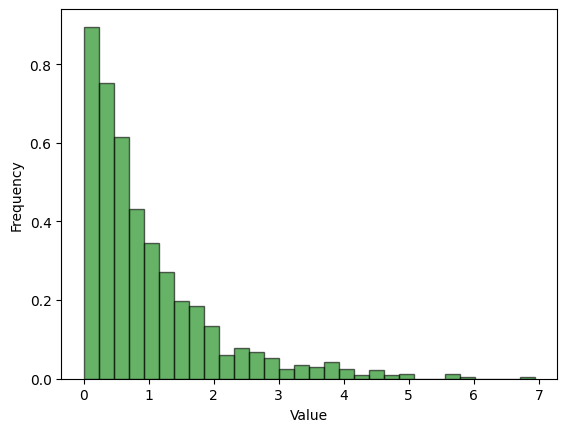
\includegraphics[width=0.5\linewidth]{./Figures/InverseCDF/histogram.png}
	\caption{Histogram of Equation \eqref{fig:inversecdfmethod} with \(\lambda = 1\) applied to \(\mathcal{U}\).}
	\label{fig:inversecdfmethod}
\end{figure}

With this picture, we can see that the histogram of the generated random numbers aligns remarkably well with the target distribution, however, we need to make more trials to be sure. We already know the theoretical mean and variance of the exponential distribution, so we can compare them with the mean of the samples while the number of trials increases.

We define the error as:

\begin{equation*} error = \frac{1}{n}\sum_{i=1}^{n} | x_i - \mu | \end{equation*}

where \(x_i\) is the \(i\)-th random number generated and \(\mu\) is the theoretical mean of the distribution.

Recall that the uniform and exponential means are:

\begin{equation*} \mu_{\mathcal{U}} = \frac{a + b}{2} \end{equation*}
\begin{equation*} \mu_{\mathcal{E}} = \frac{1}{\lambda} \end{equation*}

The Figure~\ref{fig:uniformerrorcdf} and Figure~\ref{fig:exponentialerrorcdf} shows the error to the theoretical mean as the number of trials increases for the uniform and exponential distribution.

\begin{figure}[H]
	\centering
	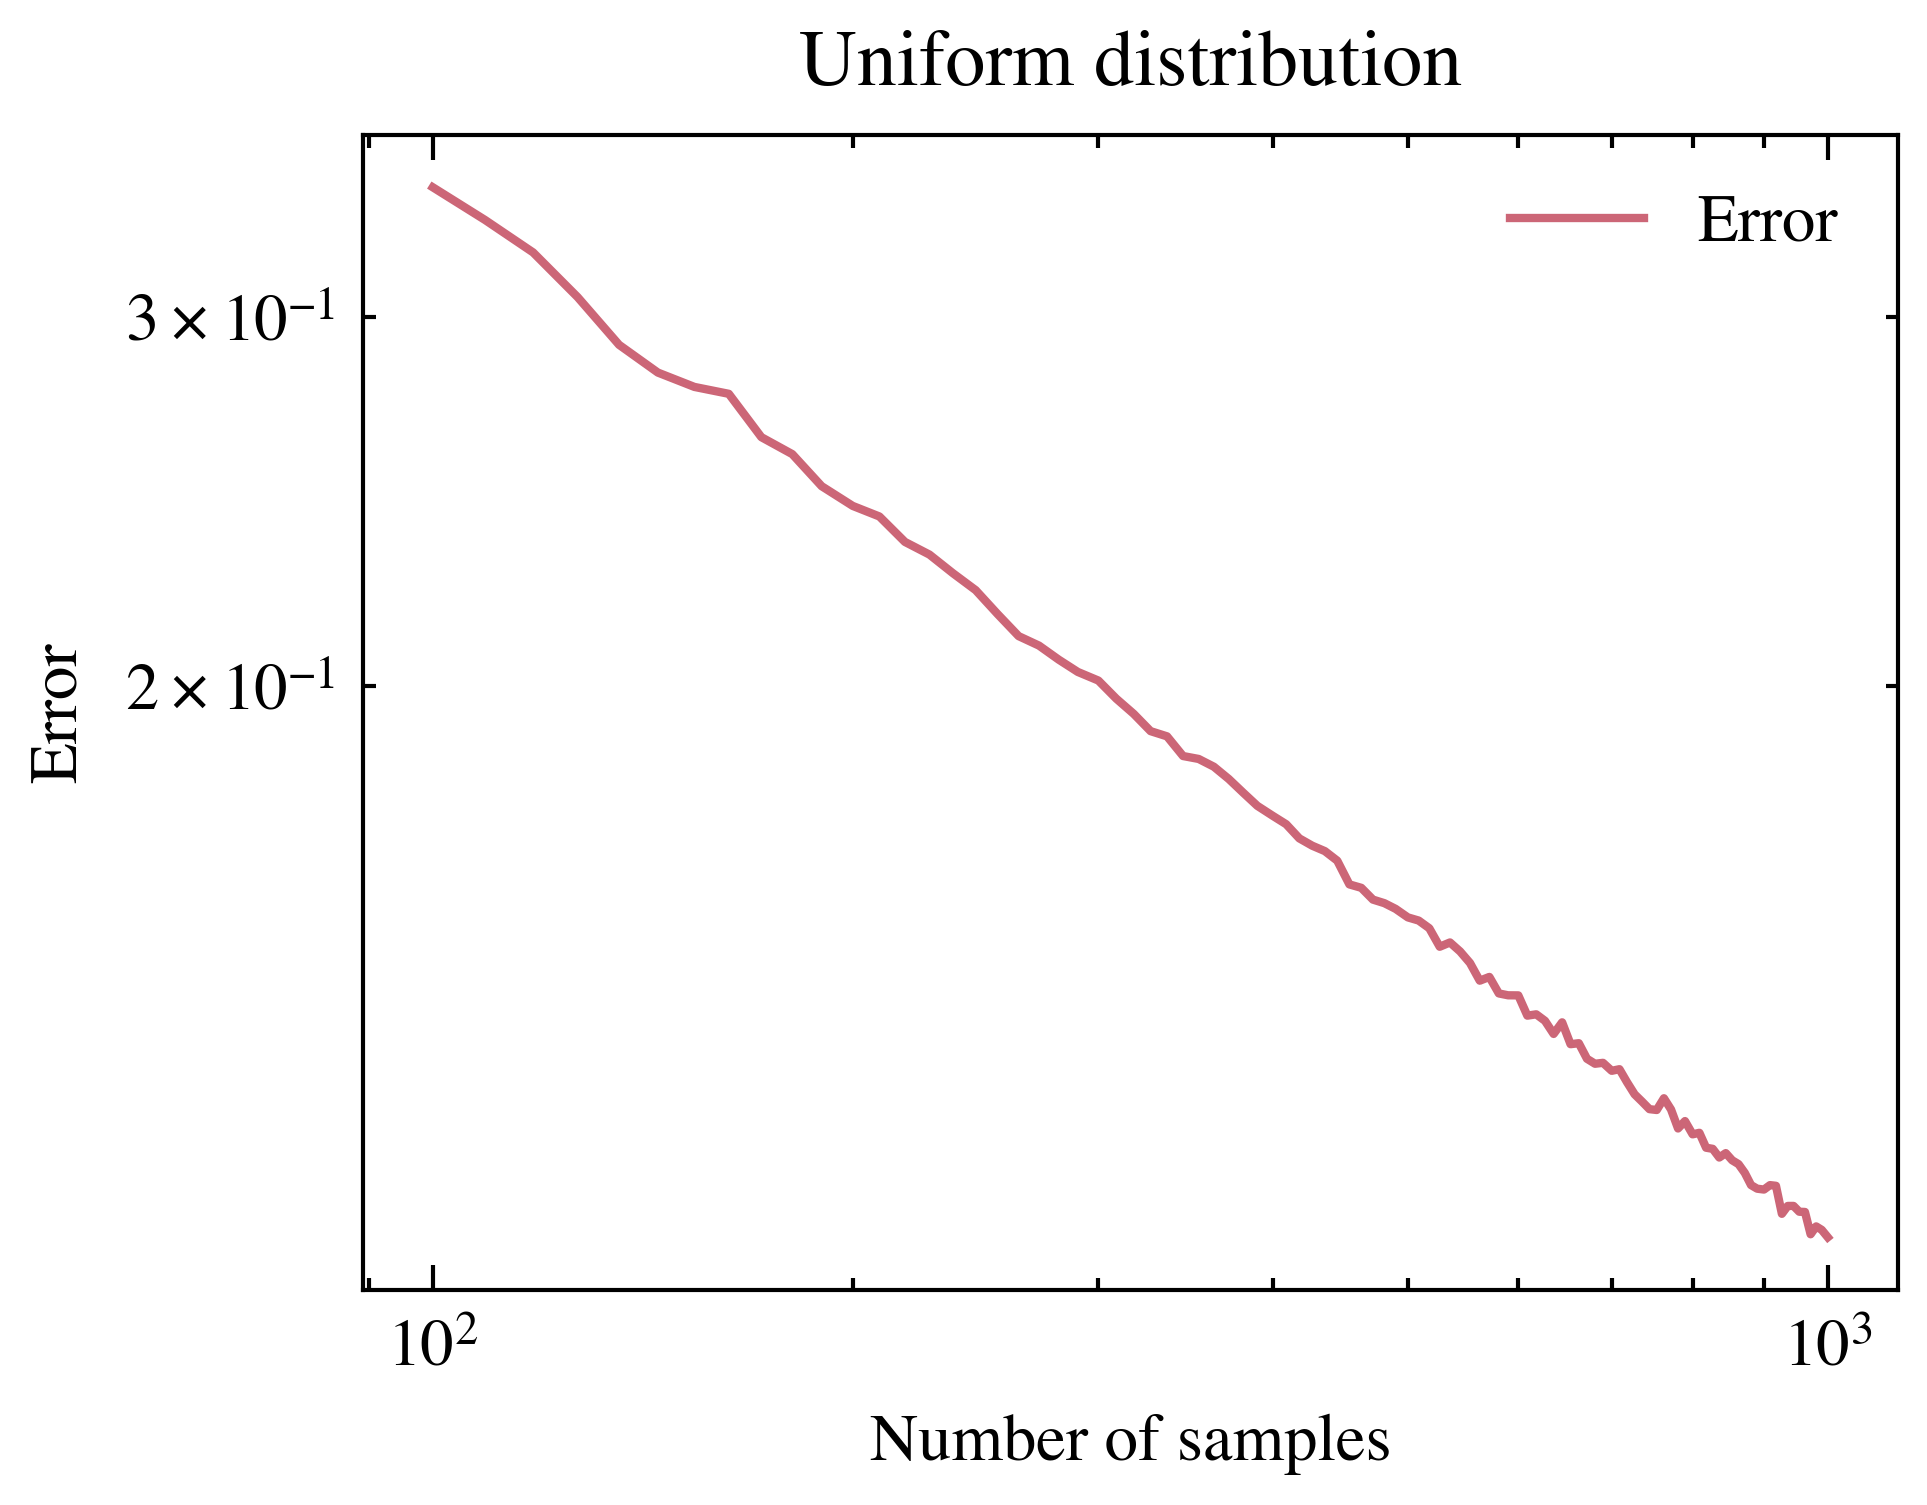
\includegraphics[width=0.5\linewidth]{./Figures/InverseCDF/uniform_error.png}
	\caption{Error to the theoretical mean as the number of trials increases for the uniform distribution. Average of 10000 trials per point.}
	\label{fig:uniformerrorcdf}
\end{figure}

\begin{figure}[H]
	\centering
	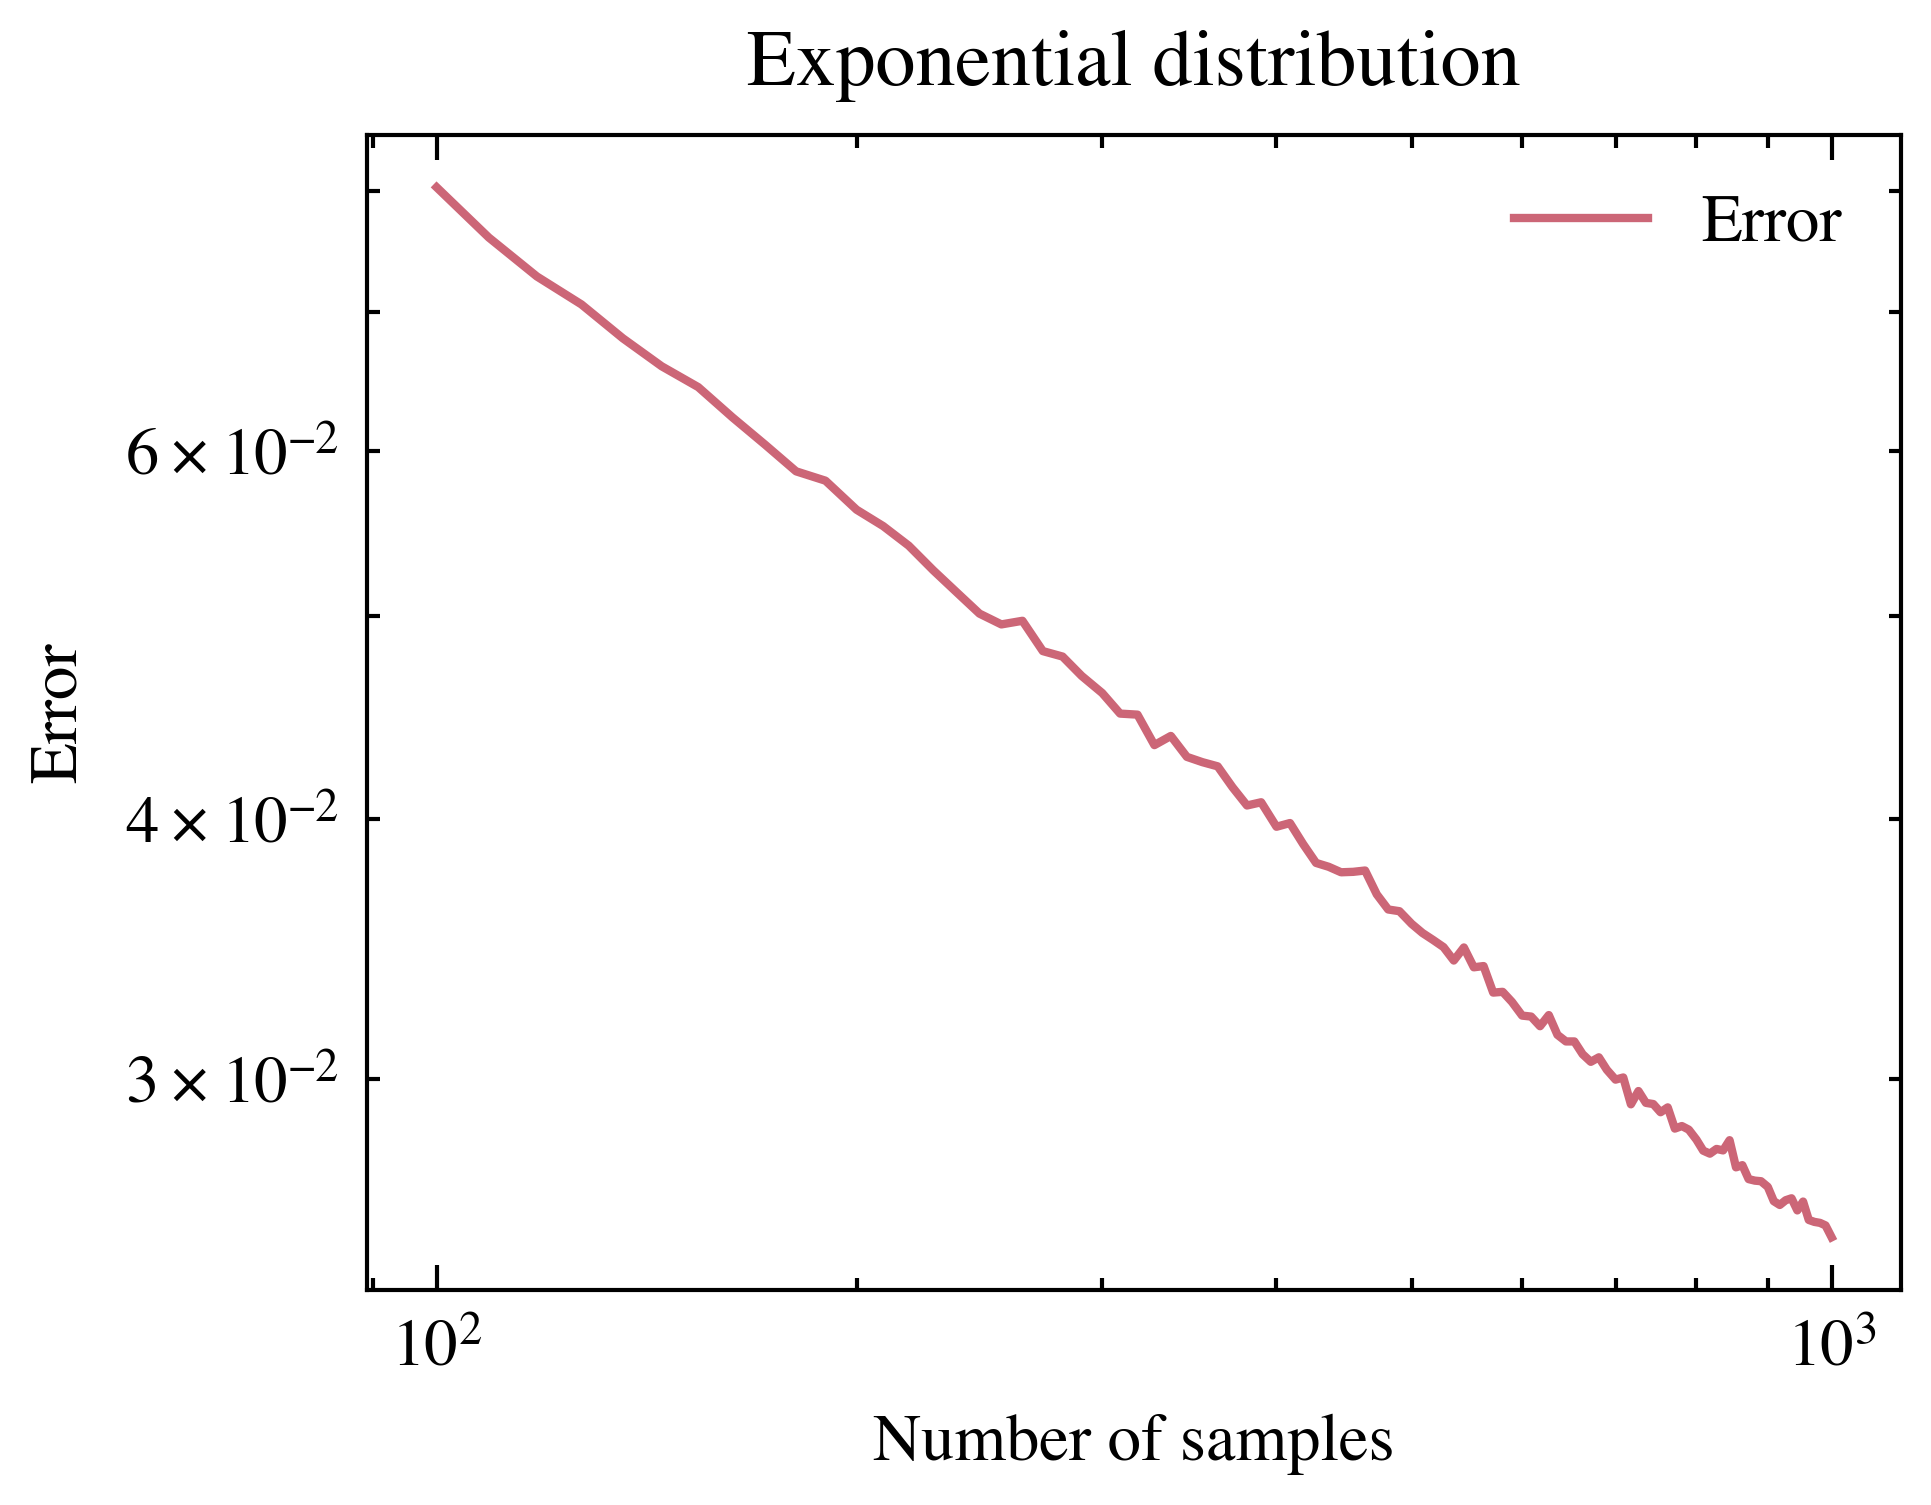
\includegraphics[width=0.5\linewidth]{./Figures/InverseCDF/exponential_error.png}
	\caption{Error to the theoretical mean as the number of trials increases for the exponential distribution. Average of 10000 trials per point.}
	\label{fig:exponentialerrorcdf}
\end{figure}

In drawing conclusions from the observed alignment of the histograms of generated random numbers with the target distribution, t  here appears to be a noteworthy relation, as evidenced by Figures~\ref{fig:uniformerrorcdf} and~\ref{fig:exponentialerrorcdf}, since the error tends to zero as the number of trials increases.



\subsection{Rejection Sampling method}
\label{sec:rejection_sampling}

The Rejection Sampling method is a method to generate pseudo-random numbers for any probability distribution given its probability density function. The idea is to generate a set of random numbers from a probability distribution that is easy to sample from and then reject the numbers that are not in the desired distribution. The Algorithm~\ref{alg:rejectionalg} is as follows:

\begin{center}
	\begin{minipage}{0.7\linewidth} % Adjust the minipage width to accomodate for the length of algorithm lines
		\begin{algorithm}[H]
			1. Generate a set of random numbers \(X \sim g(x)\) \;
			2. Generate a set of random numbers \(U \sim \mathcal{U}(0,1)\) \;
			3. If \(U \leq \frac{f(X)}{Mg(X)}\) then accept \(X\), otherwise reject \(X\) \;
			\caption{Rejection Sampling method} % Algorithm name
			\label{alg:rejectionalg}   % optional label to refer to
		\end{algorithm}
	\end{minipage}
\end{center}

Being \(g(x)\) the probability density function with which we already know how to generate random numbers, denoted as the "enveloping" distribution; \(f(x)\) the target probability density function; and \(M\) a factor we can choose manually and can be optimized. The formal explanation of why this algorithm works can be found in \cite{peng2023rejectionsampling}.

Let's see this with one example. We want to generate a set of random numbers from the following probability density function: 

\begin{equation} \label{eq:bimodal} f(x) = 0.3e^{-0.2x^2}+0.7e^{-0.2(x-5)^2} \end{equation}

\subsubsection{Selection of the "enveloping" distribution}
\label{sec:enveloping_distribution}

In this subsection we will explain the process of selecting an optimised "enveloping" distribution. In fact, we could use any distribution that envelops the desired one, but this will probably be very inefficient because there will be many samples that will not be under the objective function, so our goal is to obtain a distribution that envelops the desired one but with the smallest possible space between them. In this report we have chosen the normal distribution as the "enveloping" distribution because it is easy to sample by using the \textit{Quantile function} as the inverse CDF and applying the previous sampling method, and it is a good candidate for enveloping the desired distribution. Knowing this, we have three parameters to optimise: the mean, \(\mu\); the variance, \(\sigma\); and the scale parameter, \(M\). Note that for this problem, we have to define the bounds as \(a\), \(b\).

First of all, let's start by defining the scale parameter \(M\). In this moment, what we are looking for is a parameter that envelops the desired distribution, therefore it is a good idea to define \(M\) as follows:

\begin{equation}
	M = \max_{x \in \mathbb{R}} \frac{f(x)}{g(x)}
\end{equation}

In this way, we ensure that whatever the function is, we will envelope it. Knowing this parameter, we only have to choose \(\mu\) and \(\sigma\) in the order of minimizing \(M\). So we have a problem of optimization with two variables. The problem is the following:

\begin{equation}
	\begin{aligned}
		\min_{\mu, \sigma} \quad & M(\mu,\sigma) \\
		\textrm{s.t.} \quad & M(\mu,\sigma) = \max_{x \in \mathbb{R}} \frac{f(x)}{\frac{1}{\sqrt{2\pi\sigma^2}}e^{-\frac{(x-\mu)^2}{2\sigma^2}}} \\
		\quad &\ \sigma \geq 0, a \leq \mu \leq b \\
	\end{aligned}
	\label{eq:problemmaxmin}
\end{equation}

We can solve this problem with multiple methods. In our case, we have chosen the Nelder-Mead's method (also called downhill simplex method) \cite{doi:10.1137/S1052623496303482}.

\subsubsection{Results of the Rejection Sampling method}
\label{sec:results_rejection_sampling}

Once we have selected the "enveloping" distribution, we can apply the Rejection Sampling method. In our case, the enveloping function is the N(\(\mu \approx 3.644\) ,\(\sigma \approx 3.041\)) and the scalator parameter \(M \approx 1.545\). The Figure~\ref{fig:rejectionmethod} shows the histogram of the generated random numbers and the probability density function of the desired and the easy distribution.

\begin{figure}[H]
	\centering
	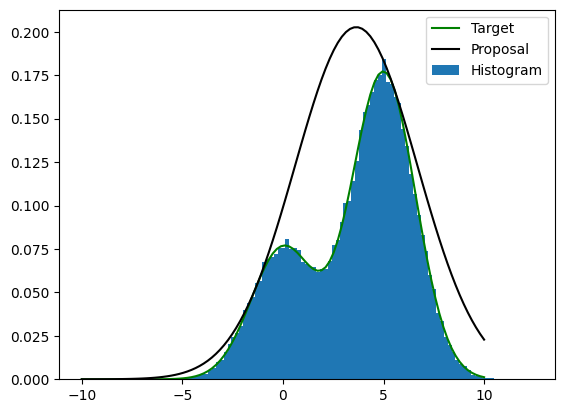
\includegraphics[width=0.5\linewidth]{./Figures/AcceptanceRejection/hist.png}
	\caption{Histogram of the generated random numbers, Equation \eqref{eq:bimodal} and PDF of \(\mathcal{N}(3.644,3.041)\) scaled by \(M \approx 1.545\).}
	\label{fig:rejectionmethod}
\end{figure}

First of all, note that the distribution chosen with the Equation~\ref{eq:problemmaxmin} fits perfectly with the target distribution. Moreover, we can see that the histogram of the generated random numbers aligns remarkably well with the target distribution. In addition to the graph display itself, we can now also compare the mean of the samples with the theoretical mean as the number of trials increases. The Figure~\ref{fig:rejectionerror} shows the error to the theoretical mean. As disclaimer, we will use the following approximation for the mean: \(\frac{1}{n}\sum_{i=1}^{n} x_i\) and the following approximation for the variance: \(\frac{1}{n}\sum_{i=1}^{n} (x_i - \bar{x})^2\).

\begin{figure}[H]
	\centering
	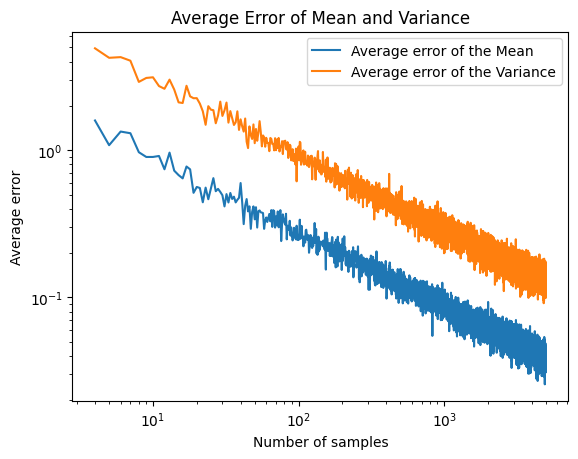
\includegraphics[width=0.5\linewidth]{./Figures/AcceptanceRejection/error_linear_regression.png}
	\caption{Error to the theoretical mean as the number of trials increases}
	\label{fig:rejectionerror}
\end{figure}

In drawing conclusions we can see that the error tends to zero as the number of trials increases, so we can conclude that the Rejection Sampling method is a good method to generate pseudo-random numbers from any probability distribution given its probability density function.

\subsection{Empirical validation of the Law of Large Numbers}
\label{sec:lln}

This section explores the empirical validation of the Law of Large Numbers, a pivotal theorem in probability theory. The Law of Large Numbers (LLN) is a fundamental theorem in probability theory, asserting that the average of a sequence of independent and identically distributed random variables with finite expected value converges to this expected value as the number of terms in the sequence increases. Formally, the theorem can be expressed as follows, extracted from \cite{jourdain2016probabilites}:

\begin{theorem}[Law of Large Numbers]
	Let $(X_j)_{j \geq 1}$ be a sequence of independent and identically distributed random variables with $\mathbb{E}(X_1^2) < + \infty$ then

	\begin{equation}
		\mathbb{E}(\bar{X}_n - \mathbb{E}(X_1))^2 = \frac{\mathrm{Var}(X_1)}{n} \xrightarrow[n \to \infty]{} 0
	\end{equation}
\end{theorem}

Given our established ability to generate random numbers reflecting specific probability distributions, we can select a distribution, generate a set of numbers corresponding to it, and then contrast the calculated averages and means of the target distribution while escalating the number of trials. Now we can define the following error:

\begin{equation} 
	error = \frac{1}{n}\sum_{i=1}^{n} (x_i - \mu)^2
\end{equation}

where \(x_i\) is the \(i\)-th random number generated and \(\mu\) is the theoretical mean of the distribution. Note that in the theorem was stated that the esperance of the difference, behaves as the variance divided by the number of trials, so we can plot the variance as the number of trials increases and calculate the slope of the regression line. If the theory is correct, the slope should be around \(-1\) since the variance of the normal distribution is \(\mathbb{V}(\bar{X}) = \frac{sigma^2}{n}\), therefore, the variance is inversely proportional to the number of variables. The Figure~\ref{fig:verificationllnlog} shows the variance as the number of variables increases and the regression line.

\begin{figure}[H]
	\centering
	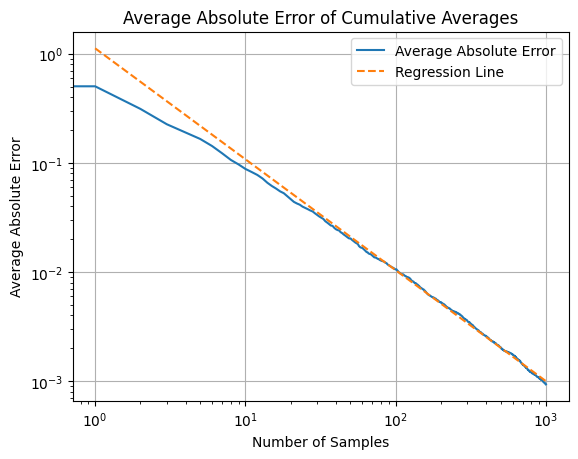
\includegraphics[width=0.5\linewidth]{./Figures/LLN/verifloglog.png}
	\caption{Logarithmic depiction of the absolute error relative to the mean. Average of 1000 trials per point.}
	\label{fig:verificationllnlog}
\end{figure}

The visual representation in Figure~\ref{fig:verificationllnlog} substantiates that the error indeed diminishes as the number of trials augments, validating the assertion of the Law of Large Numbers that the experimental mean approaches the theoretical mean with an increasing number of observations. This is further corroborated by the linear regression, which yields a slope of \(-1.000\), in alignment with the theoretical prediction.

\subsection{Empirical Validation of the Central Limit Theorem}
\label{sec:clt}

The Central Limit Theorem (CLT) posits a pivotal foundational theorem in probability theory, signifying that, irrespective of the shape of the original distribution, the distribution of sample means will approximate a normal distribution as the sample size increases. To empirically validate this theorem, we can simulate a series of random numbers from any given probability distribution and systematically calculate their mean. By repeating this process, we can construct a histogram of the means and scrutinize whether it converges to a normal distribution, aligning with the theorem's prediction. Formally, the theorem can be expressed as follows:
The Central Limit Theorem (CLT) posits a pivotal foundational theorem in probability theory, signifying that, irrespective of the shape of the original distribution, the distribution of sample means will approximate a normal distribution as the sample size burgeons. To empirically validate this theorem, we can simulate a series of random numbers from any given probability distribution and systematically calculate their mean. By perpetuating this process, we can construct a histogram of the means and scrutinize whether it converges to a normal distribution, aligning with the theorem's prediction. Formally, the theorem can be expressed as follows, extracted from \cite{jourdain2016probabilites}:

\begin{theorem}[Central Limit Theorem]
	Let $(X_j)_{j \geq 1}$ be a sequence of independent and identically distributed random variables with $\mathbb{E}(X_1^2) < + \infty$ and $\sqrt{\mathrm{Var}(X_1)} > 0$. We note $\bar{X}_n = \frac{1}{n} \sum_{j=1}^n X_j$ and $\sigma^2 = \mathrm{Var}(X_1)$. Then for $n \to \infty$,

	\begin{equation}
		\sqrt{n} \frac{\bar{X}_n - \mathbb{E}(X_1)}{\sigma} \xrightarrow[n \to \infty]{} Y \sim  \mathcal{N}(0,1)
	\end{equation}
\end{theorem}

For illustrative purposes, consider the uniform distribution on \([0,1]\), which yields a histogram as depicted in Figure~\ref{fig:verificationclt}.

\begin{figure}[H]
	\centering
	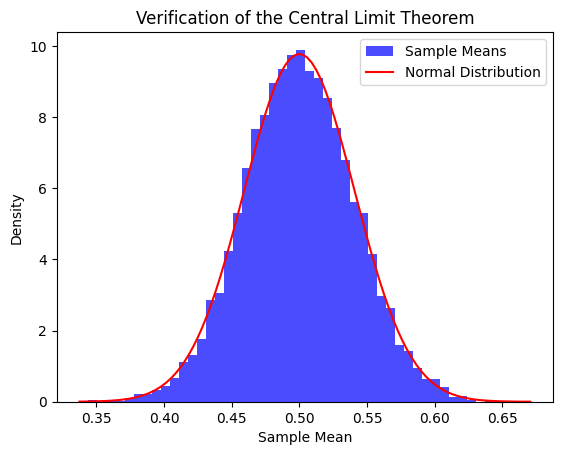
\includegraphics[width=0.5\linewidth]{./Figures/CLT/verif.png}
	\caption{Histogram illustrating the convergence of the means of the uniform distribution with $n_{samples} = 10000$}
	\label{fig:verificationclt}
\end{figure}

In congruence with the methodology espoused in previous sections, we have juxtaposed the empirical mean of the samples with the theoretical mean, progressively augmenting the number of trials. Figure~\ref{fig:meanerror} delineates the deviation from the theoretical mean, and Figure~\ref{fig:varianceerror} represents the deviation from the theoretical variance, both as functions of the number of trials. Therefore the formula of the deviation is:

\begin{equation*} error_{mean} = \frac{1}{n}\sum_{i=1}^{n} | x_i - \mu | \end{equation*}

where \(x_i\) is the \(i\)-th random number generated and \(\mu\) is the theoretical mean of the distribution.

\begin{figure}[H]
	\centering
	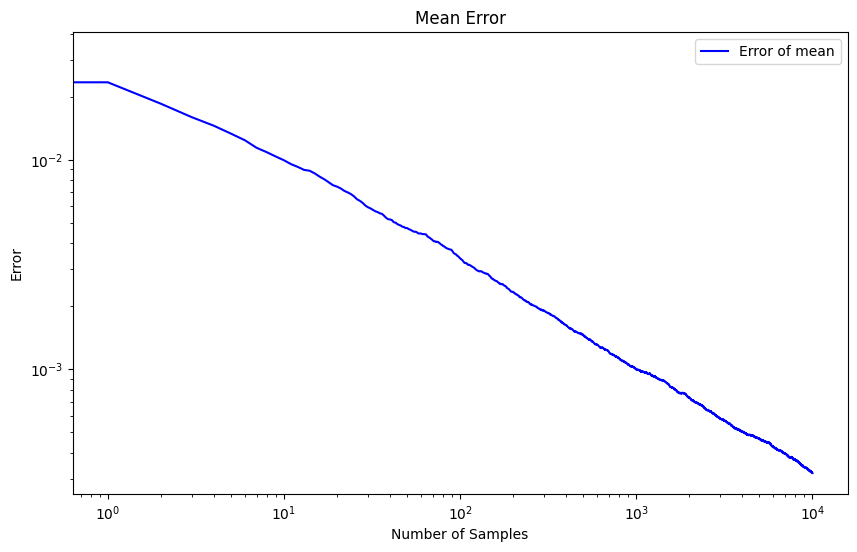
\includegraphics[width=0.5\linewidth]{./Figures/CLT/meanerror.png}
	\caption{Error from the theoretical mean as a function of the number of trials. Average of 10000 trials per point.}
	\label{fig:meanerror}
\end{figure}

And for the case of the variance:

\begin{equation*} error_{variance} = \frac{1}{n}\sum_{i=1}^{n} | x_i - \sigma^2 | \end{equation*}

where \(x_i\) is the \(i\)-th random number generated and \(\sigma^2\) is the theoretical variance of the distribution.

\begin{figure}[H]
	\centering
	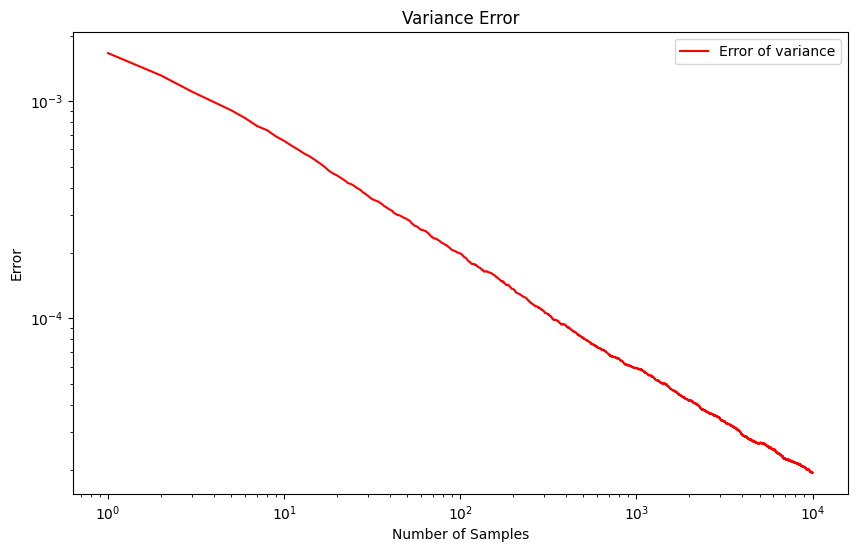
\includegraphics[width=0.5\linewidth]{./Figures/CLT/varianceerror.png}
	\caption{Error from the theoretical variance as a function of the number of trials. Average of 10000 trials per point.}
	\label{fig:varianceerror}
\end{figure}

A discernible insight gleaned from Figure~\ref{fig:meanerror} and Figure~\ref{fig:varianceerror} is the palpable decrement in deviations from the theoretical values as the trials proliferate. 

Finally, another way to validate the CLT is to plot the variance as the number of variables increases and calculate the slope of the regression line. If the theory is correct, the slope should be around \(-1\) since the variance of the normal distribution is \(\mathbb{V}(\bar{X}) = \frac{\sigma^2}{n}\), therefore the variance is inversely proportional to the number of variables. The Figure~\ref{fig:variancereg} shows the variance as the number of variables increases and the regression line.


\begin{figure}[H]
	\centering
	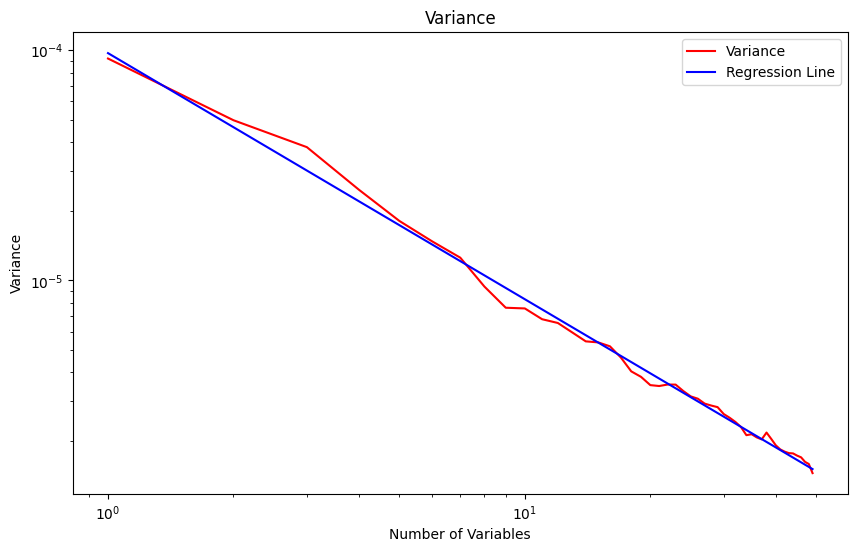
\includegraphics[width=0.5\linewidth]{./Figures/CLT/varianceslope.png}
	\caption{Deviation from the theoretical variance as a function of the number of trials. Average of 1000 trials per point.}
	\label{fig:variancereg}
\end{figure}

The slope of the regression line is \(-1\) in alignment with the theoretical prediction. This corroborates the validity of the Central Limit Theorem, as the variance of the means of the samples does indeed diminish as the number of trials increases.

\subsection{Variance reduction techniques}
\label{sec:variance_reduction}

In the theory of Monte Carlo methods, variance reduction techniques are a pivotal tool to increase the precision of the estimates of the expected value of a random variable. In this section, we will focus on three techniques: Control variates, Importance sampling and Antithetic variates. Also, we will introduce an example problem in which we will apply these techniques to compare them.

First of all, let introduce the variance reduction formally. Let $X$ be a random variable drawn from a distribution of mean \(\mathbb{E}(X) = \mu\) and finite variance \(\mathrm{Var}(X) = \sigma^2\). The estimator of the expected value of \(X\), i.e. the empirical mean of the sample, is defined as follows:

\begin{equation} 
	\label{eq:expectedvalueestimate} 
	\hat{\mathbb{E}}(X) = \frac{1}{n} \sum_{i=1}^{n} x_i
\end{equation}

So we want to reduce the variance of our estimation. Since the variance is defined as follows:

\begin{equation} 
	\label{eq:variance} 
	\mathrm{Var}(\hat{\mathbb{E}}(X)) = \frac{\mathrm{Var}(X)}{n}
\end{equation}

Consequently, we are presented with two avenues for optimization: increasing the value of \(n\), or diminishing the variance of \(X\). Assuming that \(n\) is predetermined and unalterable, our focus would then shift to minimizing the variance of \(X\).

Since we are going to introduce and compare the three techniques, first of all we need to introduce the problem we are going to solve. The problem is that we want to estimate the following integral:

\begin{equation} \label{eq:integralvariancereduction} I = \int_{0}^{1} x^2 \ dx \end{equation}

It should be noted that the selection of the integral for this demonstration was intentional; a readily solvable integral was chosen for its ease of analytical computation, allowing for a straightforward comparison with theoretical values. Nonetheless, the methods illustrated herein are equally applicable and potent for evaluating integrals that pose substantial challenges to analytical computation.

\subsubsection{Preliminaries}
\label{sec:variance_reduction_preliminaries}

First of all we have to compute which is the estimation we already can have without applying any variance reduction technique. We can compute the integral analytically. We know that the mean of the variable in a probability space is defined as follows:

\begin{equation} 
	\label{eq:directmethod} 
	\mathbb{E}(g(X)) = \int_a^b g(x)f(x) \ dx
\end{equation}

Since \(f(x) = \frac{1}{b-a}\) for the uniform distribution on \([a,b]\), we can apply Equation \eqref{eq:directmethod} to Equation \eqref{eq:integralvariancereduction} and we obtain:

\begin{equation} \label{eq:directmethodintegral} I = \int_{0}^{1} x^2 \ dx = \mathbb{E}(g(X)) = \int_0^1 x^2 \frac{1}{1-0} \ dx = \frac{1}{3} \end{equation}

So, we only have to generate a set of random numbers \(X \sim \mathcal{U}(0,1)\), apply \(g(x) = x^2\) and get the mean of the sample which is the estimate of the integral. The Figure~\ref{fig:directmethod} shows the error to the theoretical value as the number of trials increases. The error to the theoretical value is defined as:

\begin{equation*} error = \frac{1}{n}\sum_{i=1}^{n} | x_i - \mu | \end{equation*}

where \(x_i\) is the \(i\)-th random number generated and \(\mu\) is the theoretical mean of the distribution. Note that this formula will be used in all the following sections.

\begin{figure}[H]
	\centering
	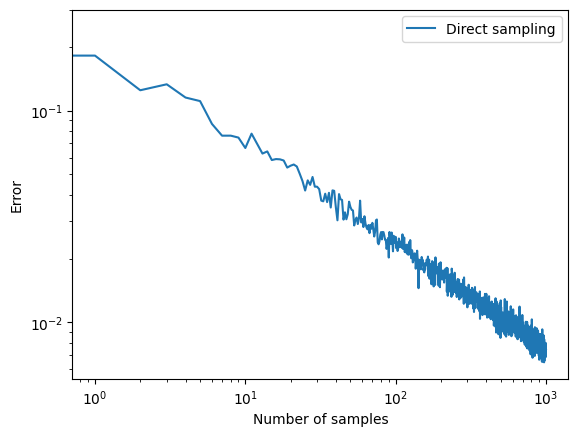
\includegraphics[width=0.5\linewidth]{./Figures/VarianceReduction/direct.png}
	\caption{Error to the theoretical value as the number of trials increases using the direct method. Average of 100 trials per point.}
	\label{fig:directmethod}
\end{figure}

Following the Equation \eqref{eq:variance}, we can compute the variance of the estimation as follows:

\begin{equation} 
	\label{eq:variancedirectmethod} 
	\mathrm{Var}(X) = \mathrm{Var}(\hat{\mathbb{E}}(X)) \ n 
\end{equation}

In this case, we have computed that \(\mathrm{Var}(X) \approx 8.977 \cdot 10^{-2}\).

\subsubsection{Control variates}
\label{sec:control_variates}

Control variates is a variance reduction technique with the following idea: Let \(\mu\) the parameter we want to estimate, and assume we have a statistic \(Y\) such that \(\mathbb{E}(Y) = \tau\). Then, we can estimate \(\mu\) by estimating \(\mathbb{E}(Y)\) as \(\hat{\mathbb{E}}(Y)\) and correcting the bias with the following formula:

\begin{equation} 
	\label{eq:controlvariates} 
	\hat{\mu} = \mu + c(\tau - \hat{\mathbb{E}}(Y)) 
\end{equation}

Being \(c\) a constant which minimize the variance of the estimation. It is computed as follows:

\begin{equation} 
	\label{eq:controlvariatesconstant} 
	c = -\frac{\mathrm{Cov}(\mu, \tau)}{\mathrm{Var}(\tau)}
\end{equation}

\begin{proof}
	Using the Equation \eqref{eq:controlvariates} we can compute the variance of the estimation as follows:
	\begin{center}
		\(\mathrm{Var}(\hat{\mu}) = \) \\

		\(\mathbb{E}[(\mu + c(\tau - \hat{\mathbb{E}}(Y)))^2] - \mathbb{E}[\mu + c(\tau - \hat{\mathbb{E}}(Y))]^2 =\) \\

		\(\mathbb{E}[\mu^2 + c^2(\tau - \hat{\mathbb{E}}(Y))^2 + 2c\sigma(\tau - \hat{\mathbb{E}}(Y))]  - \mathbb{E}[\mu]^2 - c^2\mathbb{E}[\tau - \hat{\mathbb{E}}(Y))]^2 - 2c\mathbb{E}[\sigma(\tau - \hat{\mathbb{E}}(Y))]  =\) \\

		\(\mathrm{Var}(\mu) + c^2 \mathrm{Var}(\tau) + 2cCov(\mu, \tau)\) 
	\end{center}
	Therefore, since we want to minimize the variance of the estimation, we can differentiate with respect to \(c\) and equate to zero:
	\begin{center}
		\(\frac{\partial \mathrm{Var}(\hat{\mu})}{\partial c} = 2c \mathrm{Var}(\tau) + 2\mathrm{Cov}(\mu, \tau ) = 0\) \\
	\end{center}
	And we obtain the following expression for \(c\):
	\begin{center}
		\(c = -\frac{\mathrm{Cov}(\mu, \tau)}{\mathrm{Var}(\tau)}\) 
	\end{center}


\end{proof}

In our case, we can use the knowledge of the mean of the uniform distribution to correct the bias, so in each iteration we can compute the mean of the sample of random numbers of \(\mathcal{U}(0,1)\), and knowing that the mean of the uniform distirbution is \(0.5\) we can apply Equation \eqref{eq:controlvariates} to obtain the estimate of the integral. The Figure~\ref{fig:controlvariates} shows the error to the theoretical value as the number of trials increases, i.e. the error of the estimation of the integral:

\begin{equation*}
	error = \frac{1}{n}\sum_{i=1}^{n} | x_i - \frac{1}{3} |
\end{equation*}

\begin{figure}[H]
	\centering
	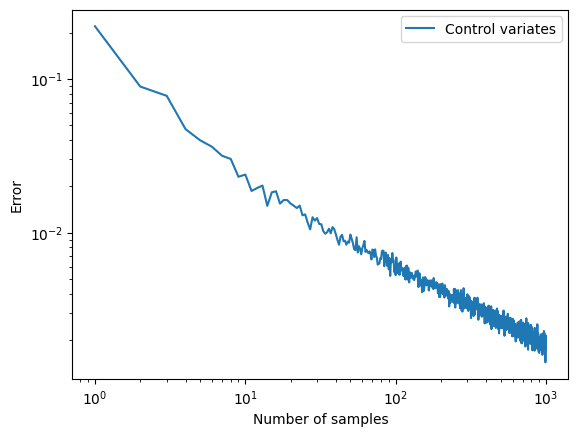
\includegraphics[width=0.5\linewidth]{./Figures/VarianceReduction/control.png}
	\caption{Error to the theoretical value as the number of trials increases using the control variates method. Average of 100 trials per point.}
	\label{fig:controlvariates}
\end{figure}

In this case, we have computed that \(\mathrm{Var}(X) \approx 5.168 \cdot 10^{-3}\).

\subsubsection{Importance sampling}
\label{sec:importance_sampling}

Importance sampling is another variance reduction technique. Instead of using the knowledge of another estimator to reduce the bias of our sample, as done in the control variates method, in this case the idea is using the knowledge of the actual function we want to integrate, so instead of using a uniform distribution, we can use another distribution that is more similar to the function we want to integrate, in order to try more samples in the areas where the function is more important. 

In our example, we know that the function is a parabola, so instead of using a sample which follows an uniform distribution, maybe we can use a distribution that fits better with the shape of the function. In this case, we have chosen \(Beta(2.9,1)\). In order to illustrate this, in the Figure~\ref{fig:beta42_f} we can see the function we want to integrate, the PDF of \(Beta(2.9,1)\) and the PDF of \(\mathcal{U}(0,1)\).

\begin{figure}[H]
	\centering
	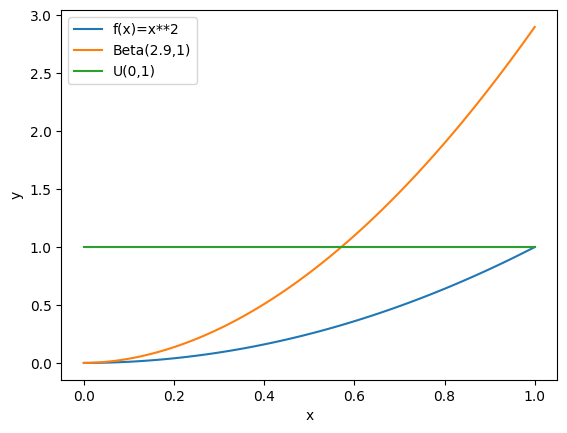
\includegraphics[width=0.5\linewidth]{./Figures/VarianceReduction/beta.png}
	\caption{Function we want to integrate, PDF of \(Beta(2.9,1)\) and PDF of \(\mathcal{U}(0,1)\)}
	\label{fig:beta42_f}
\end{figure}

As we can see, the PDF of \(Beta(2.9,1)\) fits better with the shape of the function we want to integrate, so we can expect that the error will decrease faster than the direct method and the control variates method. 

So the idea is to generate a sample of random numbers \(X \sim Beta(2.9,1)\), and take \(Y = \frac{f(X)}{g(X)}\) as the estimator of the integral, being \(f(x) = x^2\) and \(g(x)\) the PDF of \(Beta(2.9,1)\). The algorithm is as follows:

\begin{center}
	\begin{minipage}{0.7\linewidth} % Adjust the minipage width to accomodate for the length of algorithm lines
		\begin{algorithm}[H]
			1. Generate a set of random numbers \(X \sim Beta(2.9,1)\) \;
			2. Compute \(Y = \frac{f(X)}{g(X)}\) \;
			3. Compute the mean of \(Y\) as the estimator of the integral \;
			\caption{Importance Sampling method} % Algorithm name
			\label{alg:importancesampling}   % optional label to refer to
		\end{algorithm}
	\end{minipage}
\end{center}

With the error:

\begin{equation*} error = | \bar{\mathbb{E}}(X) - \frac{1}{3} | \end{equation*}

The Figure~\ref{fig:importancesampling} shows the error to the theoretical value as the number of trials increases.

\begin{figure}[H]
	\centering
	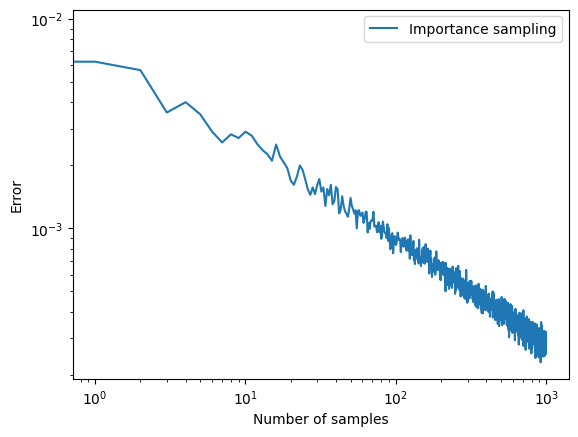
\includegraphics[width=0.5\linewidth]{./Figures/VarianceReduction/importance.png}
	\caption{Error to the theoretical value as the number of trials increases using the importance sampling method. Average of 100 trials per point.}
	\label{fig:importancesampling}
\end{figure}

In this case, we have computed that \(\mathrm{Var}(X) \approx 1.274 \cdot 10^{-4}\).

\subsubsection{Stratified sampling}
\label{sec:stratified_sampling}

The idea is to divide the interval of the stratified sampling is pretty simple. We divide the interval in \(n\) subintervals, and we generate a sample of random numbers for each subinterval. Doing this, we are trying to reduce the variance of the mean of the distribution we are considering, so the sample is more representative of the distribution. The alrogithm is as follows:

\begin{center}
	\begin{minipage}{0.7\linewidth} % Adjust the minipage width to accomodate for the length of algorithm lines
		\begin{algorithm}[H]
			1. Divide the interval in \(n\) subintervals \;
			2. Generate a set of random numbers \(X \sim \mathcal{U}(a_i,b_i)\) for each subinterval \;
			3. Compute the mean of \(X\) as the estimator of the integral \;
			\caption{Stratified Sampling method} % Algorithm name
			\label{alg:stratifiedsampling}   % optional label to refer to
		\end{algorithm}
	\end{minipage}
\end{center}

With the error:

\begin{equation*} error = | \bar{\mathbb{E}}(X) - \frac{1}{3} | \end{equation*}

The Figure~\ref{fig:stratifiedsampling} shows the error to the theoretical value as the number of trials increases.

\begin{figure}[H]
	\centering
	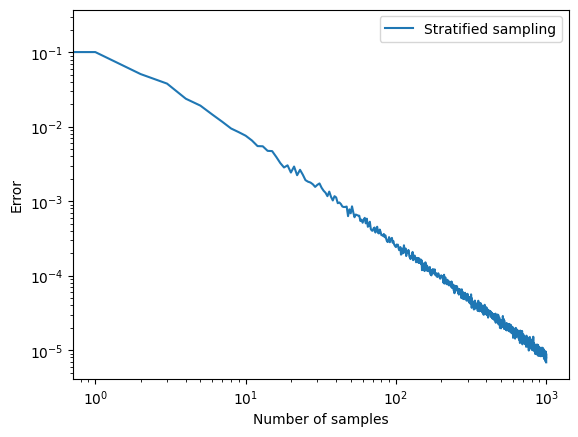
\includegraphics[width=0.5\linewidth]{./Figures/VarianceReduction/stratified.png}
	\caption{Error to the theoretical value as the number of trials increases using the stratified sampling method. Average of 100 trials per point.}
	\label{fig:stratifiedsampling}
\end{figure}

In this case, we have computed that \(\mathrm{Var}(X) \approx 1.108 \cdot 10^{-7}\).

\subsubsection{Antithetic variates}
\label{sec:antithetic_variates}

The Antithetic variates method consists on taking for each random sample, its antithetic, i.e. the symmetric with respect to the mean of the distribution. The idea is that the variance of the mean of the distribution is reduced, since the mean of the antithetic is the same as the mean of the distribution. In our case, we have generated a sample \(\mathcal{U} \sim \mathcal{U}(0,0.5)\) and its antithetic \(\mathcal{U}' = \{1 - x \ : \ x \in \mathcal{U}\}\). We can apply Equation \eqref{eq:expectedvalueestimate} to \(f(X)\) to obtain the estimate of the integral. The algorithm is as follows:

\begin{center}
	\begin{minipage}{0.7\linewidth} % Adjust the minipage width to accomodate for the length of algorithm lines
		\begin{algorithm}[H]
			1. Generate a set of random numbers \(X \sim \mathcal{U}(0,0.5)\) \;
			2. Compute the antithetic of \(X\) \;
			3. Compute the mean of \(X \bigcup X'\) as the estimator of the integral \;
			\caption{Antithetic Variates method} % Algorithm name
			\label{alg:antitheticvariates}   % optional label to refer to
		\end{algorithm}
	\end{minipage}
\end{center}

With the error:

\begin{equation*} error = | \bar{\mathbb{E}}(X) - \frac{1}{3} | \end{equation*}

The Figure~\ref{fig:antitheticvariates} shows the error to the theoretical value as the number of trials increases.

\begin{figure}[H]
	\centering
	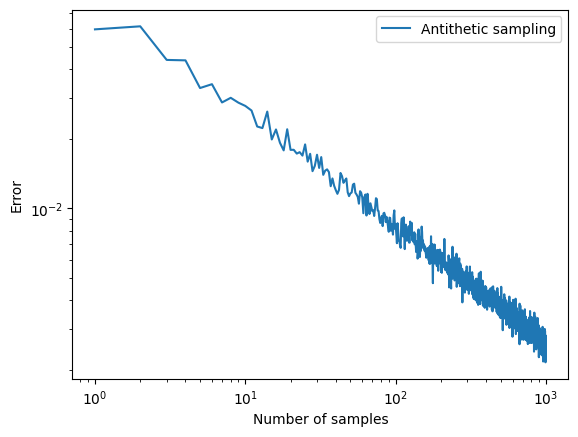
\includegraphics[width=0.5\linewidth]{./Figures/VarianceReduction/antithetic.png}
	\caption{Error to the theoretical value as the number of trials increases using the antithetic variates method. Average of 100 trials per point.}
	\label{fig:antitheticvariates}
\end{figure}

In this case, we have computed that \(\mathrm{Var}(X) \approx 1.178 \cdot 10^{-2}\).

\subsubsection{Comparative Review}
\label{sec:comparative_review}

Having looked at the methods and confirmed the convergence of each approach described in this study, we now turn to a more focused comparison of these techniques. The goal is simple: find out which method works best for our specific problem. See Figure~\ref{fig:comparisonvariancereduction} for a visual representation of the error in relation to the theoretical value as we increase the number of trials for each method.

\begin{figure}[H]
\centering
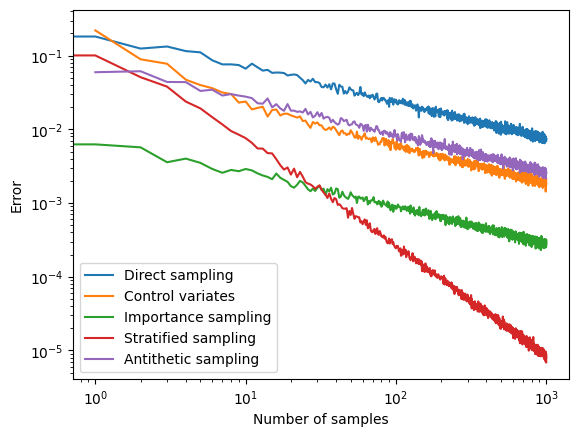
\includegraphics[width=0.5\linewidth]{./Figures/VarianceReduction/comparison.png}
\caption{Error variation with increased trials for each method.}
\label{fig:comparisonvariancereduction}
\end{figure}

Note that the error was defined as follows:	

\begin{equation*} error = | \bar{\mathbb{E}}(X) - \frac{1}{3} | \end{equation*}

Looking at the data, it’s clear that stratified sampling takes the lead with its quicker convergence compared to the other methods. However, claiming it as the undisputed champion would be premature, especially when we’ve explored just one problem. To firm up this initial finding, we need to dig deeper and explore a variety of problems.

But before moving on to look at more problems, let's look at the comparative table of variances for each method:

\begin{center}
	\begin{tabular}{ |p{5cm}||p{3cm}|p{3cm}|p{3cm}|  }
		\hline
		Method & Variance \\
		\hline
		\hline
		Direct sampling   			& \(8.977194 \cdot 10^{-2}\) \\
		\hline
		Control variates sampling 	& \(5.168373 \cdot 10^{-3}\) \\
		\hline
		Importance sampling      	& \(1.274508 \cdot 10^{-4}\) \\
		\hline
		Stratified sampling       	& \(1.107865 \cdot 10^{-7}\) \\
		\hline
		Antithetic sampling      	& \(1.178326 \cdot 10^{-2}\) \\
		\hline
	\end{tabular}
\end{center}

Recall that the formula used to compute the variance is:

\begin{equation*} \mathrm{Var}(X) = \mathrm{Var}(\hat{\mathbb{E}}(X)) \ n \end{equation*}

With a sample size of \(n = 1000\).

Analyzing the table, we discern significant disparities in variance between the different sampling methods, accentuating the prominence of stratified sampling, which registers the minimal variance,. This numerical inferiority in variance corroborates the preliminary observation about its superior convergence rate, offering more stable and reliable estimates. Stratified sampling outperformed other methods in our study primarily due to its targeted approach of dividing the population into homogeneous strata. This division ensures proportional representation of all subgroups, reducing sampling bias and variance within each stratum. Consequently, it yields more accurate and representative results. Furthermore, by adjusting the sample size within each stratum based on variability, stratified sampling enhances overall efficiency and precision. These methodological strengths contribute to its superior performance in terms of reliability and convergence rates, especially in diverse and complex datasets. Contrastingly, direct sampling exhibits the maximum variance, revealing its comparative inefficiency and instability in procuring estimates for this specific problem. The remaining methods, while overshadowed by the efficacy of stratified sampling, still exhibit markedly lower variances than direct sampling.

Next, we'll broaden our investigation to a more complex problem, applying the methods we’ve discussed to estimate the following integrals:

\begin{equation} 
	\label{eq:integralvariancereduction1} 
	\text{Parabola} = \int_{0}^{1} x^2 \ dx 
\end{equation}

\begin{equation} 
	\label{eq:integralvariancereduction2} 
	\text{Gaussian} = \int_{0}^{1} e^{-x^2} \ dx
\end{equation}

\begin{equation} 
	\label{eq:integralvariancereduction3} 
	\text{Sine} = \int_{0}^{1} \sin(x) \ dx
\end{equation}

\begin{equation} 
	\label{eq:integralvariancereduction4} 
	\text{Polynomial} = \int_{0}^{1} x^3 - 2x^2 + x \ dx
\end{equation}

\begin{equation} 
	\label{eq:integralvariancereduction5} 
	\text{Exponential} = \int_{0}^{1} e^x \ dx
\end{equation}

Using these examples, we can now draw comparisons between the methods in a broader context. Figure~\ref{fig:comparisonvariancereduction2} illustrates the error of each method applied to each function.

This error is defined as:

\begin{equation*} error = | \ method(f, a, b, iters) - \int_a^b{f dx} \ | \end{equation*}

where \(method\) is the method we are using, \(f\) is the function we are integrating, \(a\) and \(b\) are the limits of the integral and \(iters\) is the number of iterations we are using, in this case \(iters = 1000\).

\begin{figure}[H]
\centering
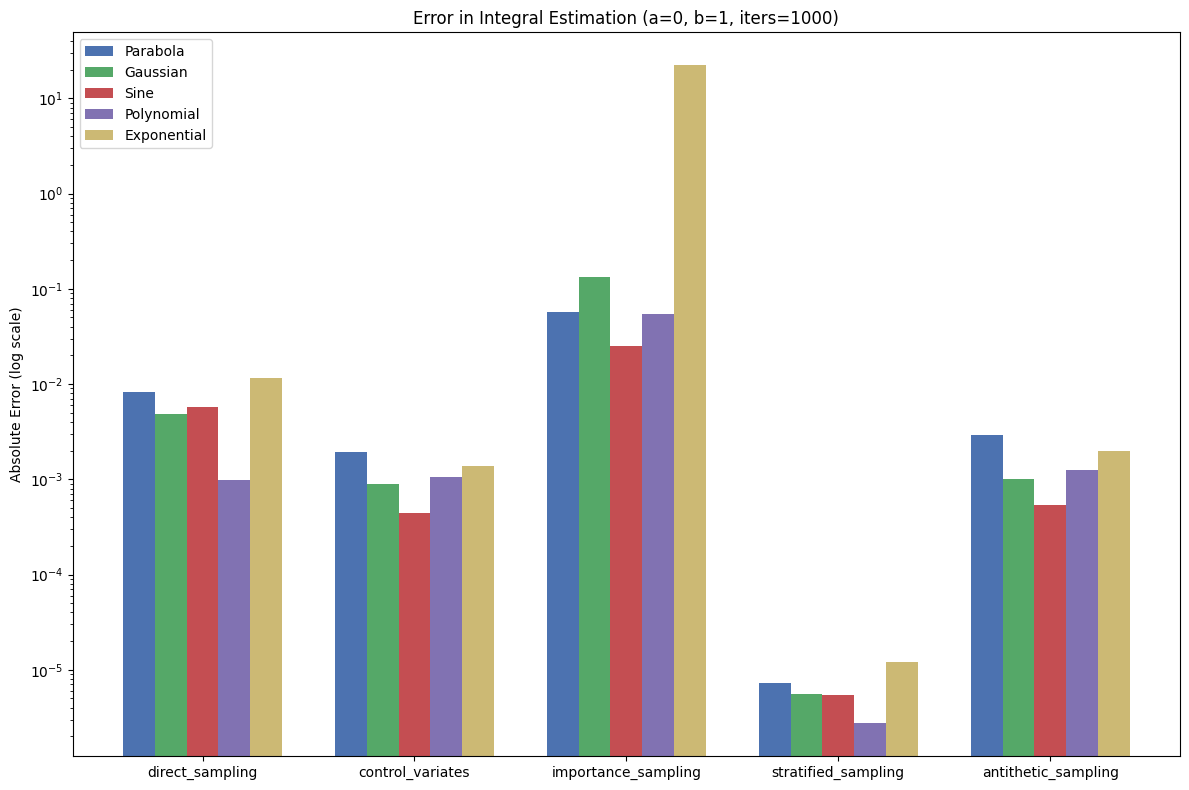
\includegraphics[width=0.8\linewidth]{./Figures/VarianceReduction/comparison2.png}
\caption{Method-wise error in each function.}
\label{fig:comparisonvariancereduction2}
\end{figure}

Note that in the cace of importance sampling, we have used the gaussian distribution as the sampling distribution, therefore the error could be higher than the other methods, since the gaussian distribution might not be the best sampling distribution for all the functions. To conclude, we can say that the stratified sampling method is the best method for this problem, since it has the lowest error in all the functions. 

\section{Hamiltonian dynamics}
\label{sec:hamiltonian_dynamics}

This section delves into the realm of Hamiltonian dynamics, beginning with an in-depth exploration of symplectic schemes in Section 2.1 (\ref{sec:symplectic_schemes}). This section starts with a discussion on the analytical solution in Section 2.1.1 (\ref{sec:analytical_solution}), setting the groundwork for understanding symplectic integration methods.

In Section 2.1.2 (\ref{sec:euler_method}), the focus shifts to the Euler method, detailing its application and significance in Hamiltonian systems. Following this, Section 2.1.3 (\ref{sec:failure_standard_methods}) discusses the limitations and failures of standard methods in this context, highlighting the need for more sophisticated approaches.

Section 2.1.4 (\ref{sec:constructing_symplectic_schemes}) addresses the construction of symplectic schemes, a crucial step for accurate simulations in Hamiltonian dynamics. This is further expanded in Section 2.1.5 (\ref{sec:symplectic_euler_method}), which specifically examines the Symplectic Euler method. A detailed Linear Stability Analysis of the Symplectic Euler scheme is then presented in Section 2.1.5.1 (\ref{sec:linear_stability_symplectic_euler}).

The narrative continues with the Stormer-Verlet method in Section 2.1.6 (\ref{sec:stormer_verlet_method}), another important technique in symplectic integration, followed by a Linear Stability Analysis of the Verlet scheme in Section 2.1.6.1 (\ref{sec:linear_stability_verlet}). Section 2.1.7 (\ref{sec:backward_error_analysis}) concludes this part with a discussion on Backward Error Analysis, providing insights into the error characteristics of symplectic integrators.

Section 2.2 (\ref{sec:solar_system_simulation}) shifts the focus to the practical application of these concepts in simulating the solar system. Section 2.2.1 (\ref{sec:modeling_solar_system}) begins with modeling gravitational dynamics, followed by the implementation of the Störmer-Verlet scheme in Section 2.2.2 (\ref{sec:stormer_verlet_scheme_gravitational_dynamics}). The implementation details of these models are further elaborated in Section 2.2.3 (\ref{sec:implementation_solar_system}), with two experiments: Experiment 1 in Section 2.2.3.1 (\ref{sec:expanding_n_body_problem}) expands to the N-Body problem, and Experiment 2 in Section 2.2.3.2 (\ref{sec:using_symplectic_euler_method}) utilizes the Symplectic Euler Method, providing practical insights into their application in complex dynamical systems.

\subsection{Introduction to Hamiltonian dynamics}
\label{sec:introduction_hamiltonian_dynamics}

Hamiltonian dynamics, also called "Hamiltonian mechanics", is a reformulation of the clasical mechanics which describes the temporal evolution of a physical system in terms of pairs of variables: the generalized coordinates \(q_i\) and their momenta \(p_i\).

\begin{equation*}
	p(t) = \begin{bmatrix} p_1(t) \\ p_2(t) \\ \vdots \\ p_n(t) \end{bmatrix} \; \ 
	q(t) = \begin{bmatrix} q_1(t) \\ q_2(t) \\ \vdots \\ q_n(t) \end{bmatrix} \;
\end{equation*}

In this section we consider the time evolution of a isolated system described at a microscopic level, i.e. a system of particles. The state of the system is described by the position of the particles \(q_i\) and their momenta \(p_i\). We denote \(D\) the dimension of the positions and momenta variables. Therefore \(D = 3N\) when the system is composed of \(N\) particles in a 3-dimensional physical space. Also, we assume that for the system there is a function \(H(q,p,t)\) which describes the energy of the system.

The Hamiltonian dynamics is defined by the following equations:

\begin{equation} 
	\label{eq:hamiltoniandynamics1} 
	\begin{cases}
		\frac{dq(t)}{dt} = \nabla_p H(q(t), p(t)) \\
		\frac{dp(t)}{dt} = -\nabla_q H(q(t), p(t))
	\end{cases}
\end{equation}

With initial condition \(p(0)=p^0, \ q(0)=q^0\) that should be provided. Now, introducing the following matrix:

\begin{equation*}
	J = \begin{bmatrix} 0 & I \\ -I & 0 \end{bmatrix}
\end{equation*}

And denoting \(y = (q,p)\), we can rewrite the Hamiltonian dynamics equations as follows:

\begin{equation} 
	\frac{dy}{dt} = J \nabla H(y) = J \begin{bmatrix} \nabla_q H(y) \\ \nabla_p H(y) \end{bmatrix}
	\label{eq:hamiltoniandynamics2} 
\end{equation}

A Hamiltonian function is the sum of the kinetic energy and the potential energy of the system:

\begin{equation*}
	H(q,p) = K(p) + V(q)
\end{equation*}

A very common physical interpretation of the Hamiltonian function is the following:

\begin{equation*}
	H(q,p) = V(q) + \frac{1}{2} p^T M^{-1} p
\end{equation*}

Where \(M\) is the mass matrix of the system, i.e. \(M = \mathrm{diag}(m_1, m_2, ..., m_n)\) with \(m_i\) the mass of the \(i\)-th particle, note that we are supposing that the mass is stable over time. In this case, we can reformulate the Hamiltonian dynamics equations as follows:

\begin{equation} 
	\begin{cases}
		\frac{dq(t)}{dt} = M^{-1} p(t) \\
		\frac{dp(t)}{dt} = -\nabla_q V(q(t))
	\end{cases}
	\label{eq:hamiltoniandynamics3}
\end{equation}

Therefore, if we consider this equations in terms of positions we get:

\begin{equation*} 
	M\frac{d^2q(t)}{dt^2} = -\nabla_q V(q(t))
\end{equation*}

Which is the Newton's second law of motion. So, we can see that the Hamiltonian dynamics is a generalization of the Newton's second law of motion.

One of the most important property of the Hamiltonian dynamics is the following:

\begin{theorem}[Conservation of energy]
	Let \(H(q,p)\) be the Hamiltonian function of a system. Then, the energy of the system is conserved over time, i.e. \(H(q(t),p(t)) = H(q^0,p^0)\) for all \(t\).
\end{theorem}

\begin{proof}
	Deriving the Hamiltonian function with respect to time we get:

	\begin{gather*}
		\frac{dH}{dt} = \frac{\partial H}{\partial q} \frac{dq}{dt} + \frac{\partial H}{\partial p} \frac{dp}{dt} = \\ 
		= \nabla_q H \frac{dq}{dt} + \nabla_p H \frac{dp}{dt} = \\ 
		= \nabla_q H J \nabla_p H - \nabla_p H J \nabla_q H = 0
	\end{gather*}

	Since the hamiltonian \(H\) is defined as the total energy of the system, we can conclude that the energy of the system is conserved over time.
\end{proof}

\subsection{Symplectic schemes}
\label{sec:symplectic_schemes}

In this section we will introduce the symplectic schemes, which are a family of numerical methods to solve the Hamiltonian dynamics equations. The idea is to discretize the Hamiltonian dynamics equations \eqref{eq:hamiltoniandynamics2} in order to obtain a numerical approximation of the solution. The symplectic schemes are a family of numerical methods which preserve the symplectic structure of the Hamiltonian dynamics equations, i.e. the energy of the system is conserved over time.

\begin{definition}
	For an open set \(U \subset \chi \), a mapping \(g: U \rightarrow \mathbb{R}^{2D}\) of class \(C^1\) is symplectic if \(\nabla g(q,p)\) satisfies
	\[
		(\nabla g)^T J \nabla g = J, \ \ \forall (q,p) \in U
	\]
\end{definition}

\subsubsection{Analytical solution}
\label{sec:analytical_solution}

Let us introduce a simple example problem to illustrate the symplectic schemes: the harmonic oscillator. The harmonic oscillator is a system composed of a particle of mass \(m\) attached to a spring with spring constant \(k\). The position of the particle is denoted by \(q(t)\). The potential energy of the system is defined as follows:

\begin{equation*}
	V(q) = \frac{1}{2} k q^2
\end{equation*}

Therefore, the Hamiltonian function of the system is defined as follows:

\begin{equation}
	H(q,p) = \frac{1}{2m} p^2 + \frac{1}{2} k q^2
	\label{eq:hamiltonianharmonicoscillator}
\end{equation}

Applying this Hamiltonian function to the Hamiltonian dynamics equations \eqref{eq:hamiltoniandynamics2} we obtain the following equations:

\begin{equation*}
	\begin{cases}
		\frac{dq(t)}{dt} = \frac{1}{m} p(t) \\
		\frac{dp(t)}{dt} = -k q(t)
	\end{cases}
\end{equation*}

Let's proceed step by step to solve the given system of differential equations for the harmonic oscillator. We are given the Hamiltonian:

\[
H(q,p) = \frac{1}{2m} p^2 + \frac{1}{2} k q^2
\]

And the Hamilton's equations:

\[
	\begin{cases}
		\frac{dq(t)}{dt} = \frac{1}{m} p(t) \\
		\frac{dp(t)}{dt} = -k q(t)
	\end{cases}
\]

We can combine the two first-order differential equations into a single second-order differential equation by substituting the expression for \( \dot{x}(t) \) into the derivative \( \dot{p}(t) \). Substituting \( \dot{x}(t) = \frac{1}{m} p(t) \) into the derivative of the second equation gives us:

\[
	\frac{d^2q(t)}{dt^2} = -\frac{k}{m} q(t)
\]

This is a second-order homogeneous linear differential equation.

To solve this second-order differential equation, we can use the characteristic equation method. Assume a solution of the form:

\[
	q(t) = e^{rt}
\]

where \( r \) is a constant to be determined. Substituting this into the second-order equation gives:

\[
	r^2 e^{rt} + \frac{k}{m} e^{rt} = 0
\]

Since \( e^{rt} \) is never zero, we can divide through by it to get the characteristic equation:

\[
	r^2 + \frac{k}{m} = 0
\]

Solving for \( r \) gives us:

\[
	r = \pm i \sqrt{\frac{k}{m}}
\]

where \( i \) is the imaginary unit.

Given that the roots are complex, the general solution of the equation is:

\[
	\begin{cases}
		q(t) = A \cos(\omega t) + B \sin(\omega t) \\
		p(t) = -m \omega A \sin(\omega t) + m \omega B \cos(\omega t)
	\end{cases}
\]

where \( A \) and \( B \) are arbitrary constants determined by initial conditions and \( \omega = \sqrt{\frac{k}{m}} \) is the angular frequency of the oscillator. In order to determine the constants \( A \) and \( B \), we need initial conditions. Specifically, we need the initial position \( x(0) \) and initial velocity \( \dot{x}(0) \). Let's say, for example:

\[
q(0) = q_0 \quad \text{and} \quad \dot{q}(0) = v_0
\]

Substituting these into the general solution and its derivative gives:
\[
q_0 = A \quad \text{and} \quad v_0 = B \omega
\]

Thus, if initial conditions are provided, \( A \) and \( B \) can be determined to give the particular solution for the system. For example, if we take \(x_0 = 1\) and \(v_0 = 0\), we get that \(A = 1\) and \(B = 0\). Therefore, the solution of the harmonic oscillator is:

\[
	\begin{cases}
		q(t) = \cos(\omega t) = \cos(\sqrt{\frac{k}{m}} t) \\
		p(t) = -m \omega \sin(\omega t) = -\sqrt{km} \sin(\sqrt{\frac{k}{m}} t)
	\end{cases}
\]

The Figure~\ref{fig:harmonicoscillator} shows the phase space of the harmonic oscillator with \(k = 1\) and \(m = 1\).

\begin{figure}[H]
	\centering
	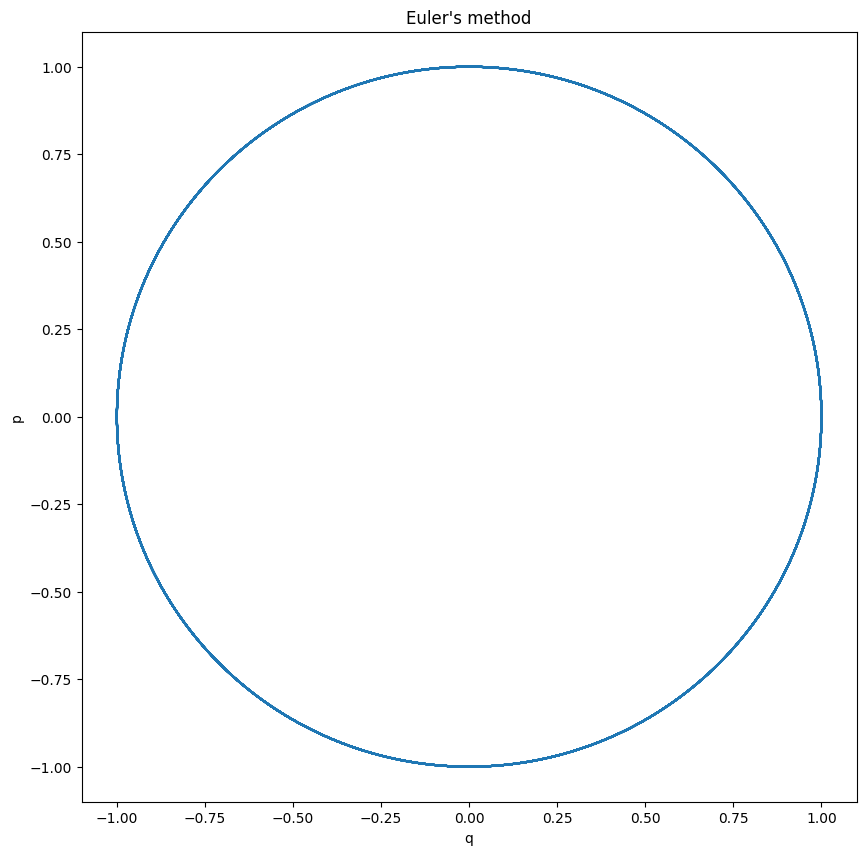
\includegraphics[width=0.5\linewidth]{./Figures/Sympletic/phaseanalytics.png}
	\caption{Phase space of the harmonic oscillator with \(k = 1\) and \(m = 1\) and initial conditions \(q_0 = 1\) and \(v_0 = 0\).}
	\label{fig:harmonicoscillator}
\end{figure}


\subsubsection{Euler method}
\label{sec:euler_method}

The Euler method is a numerical method to solve ordinary differential equations. The idea is to discretize the differential equation in order to obtain a numerical approximation of the solution. The Euler method discretizes the differential equation as follows:

\begin{equation}
	\begin{cases}
		p_{t+ \Delta t} &= p_t - \Delta t \frac{\partial H}{\partial q}(q_t, p_t) = p_t - \Delta t \nabla_q V(q_t) \\
		q_{t+ \Delta t} &= q_t + \Delta t \frac{\partial H}{\partial p}(q_t, p_t) = q_t + \Delta t M^{-1} p_t
	\end{cases}
	\label{eq:euler}
\end{equation}

Being \(\Delta t\) the time step of the discretization. Applying this sequence to the harmonic oscillator, which equations are described in \eqref{eq:hamiltonianharmonicoscillator}, we obtain the following phase space:

\begin{figure}[H]
	\centering
	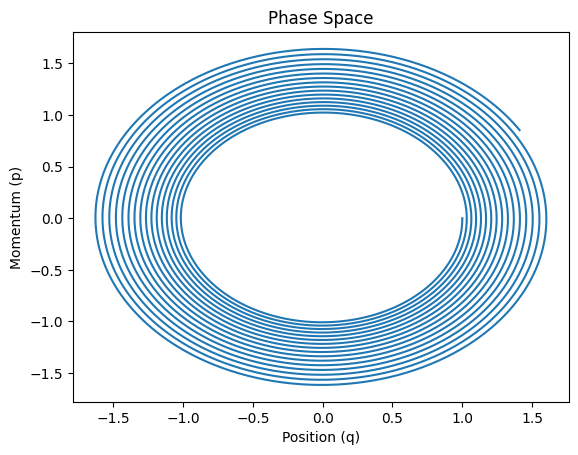
\includegraphics[width=0.5\linewidth]{./Figures/Sympletic/eulerphase1.png}
	\caption{Phase space of the harmonic oscillator using the Euler method with \(\Delta t = 0.01\).}
	\label{fig:hamiltonianharmonicoscillator}
\end{figure}

As we can discern, this phace space is not even near to the real phase space of the harmonic oscillator. The Figure~\ref{fig:hamiltonianharmonicoscillator} shows the phase space of the harmonic oscillator using the Euler method with \(\Delta t = 0.1\). We can see that the phase space is not a closed curve, which is the correct behaviour of the harmonic oscillator. Also, the energy is not conserved over time, which is another property of the harmonic oscillator. The Figure~\ref{fig:hamiltonianharmonicoscillatorenergy} shows the energy of the harmonic oscillator using the Euler method with \(\Delta t = 0.1\).

\begin{figure}[H]
	\centering
	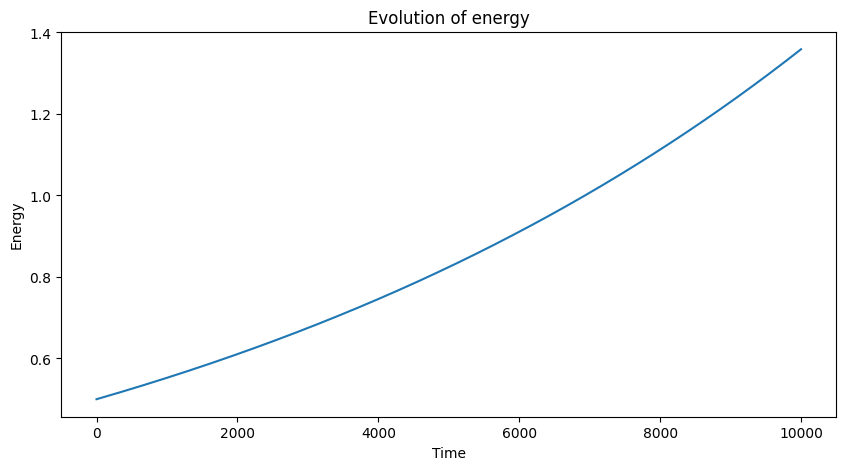
\includegraphics[width=0.5\linewidth]{./Figures/Sympletic/eulerenergy1.png}
	\caption{Energy of the harmonic oscillator using the Euler method with \(\Delta t = 0.01\).}
	\label{fig:hamiltonianharmonicoscillatorenergy}
\end{figure}

As we can see, the energy is not conserved over time, which is another property of the harmonic oscillator. The energy is increasing over time, which is not the correct behaviour of the harmonic oscillator. With this results we can conclude that the Euler method is not a good method to solve the Hamiltonian dynamics equations. This is a consequence of the fact that the Euler method does not preserve the symplectic structure of the Hamiltonian dynamics equations. Therefore, in the next section we will introduce a new method that preserves the symplectic structure of the Hamiltonian dynamics equations which is a slight modification of the Euler method.

\subsubsection{Failure of standard methods}
\label{sec:failure_standard_methods}

As we alredy know, the Hamiltonian dynamics is a standard ordinal differential equation (ODE), so it can be approximated by any standard integration scheme. However, as we saw using the Euler scheme, the energy increases over the time so it doesn't work. To provide a further view of this, in this section, we want to introduce the mathematical approach to see why this methods are failing. Considering again the problem of the harmonic oscillator, whose Hamiltonian is provided in \ref{eq:hamiltonianharmonicoscillator}. And taking the euler scheme given in \ref{eq:euler} we can rewrite it to:

\[
	\begin{pmatrix} p^{n+1} \\ q^{n+1} \end{pmatrix} = A \begin{pmatrix} p^{n} \\ q^{n} \end{pmatrix}
\]

Being \(A = \begin{pmatrix} 1 & -k\Delta t \\ \frac{1}{m} \Delta t & 1  \end{pmatrix}\). Now we diagonalize this matrix, so we obtain that its eigenvalues are:

\[
	\lambda_1 = 1 + i\Delta t\sqrt{\frac{k}{m}} = i + i \Delta t \omega, \quad
	\lambda_2 = 1 - i\Delta t\sqrt{\frac{k}{m}} = i - i \Delta t \omega
\]

Since \(\lambda_1 \lambda_2 = 1 + (\Delta t \omega)^2 > 1\) the energy exponentially increases in the time. Following this way of reasoning, it can be easily checked that the Runge-Kutta scheme and the implicit Euler scheme also fail. So the next step of the project is to construct schemes that can conserve the energy.


\subsubsection{Constructing Symplectic Schemes}
\label{sec:constructing_symplectic_schemes}

To develop an integrator, we split the Hamiltonian \(H(q,p)\) into simpler components:

\begin{equation*}
	H(q,p) = H_1(q,p) + H_2(q,p)
\end{equation*}

With:
\begin{align*}
	H_1(q,p) & = \frac{1}{2} p^T M^{-1} p \quad (\text{kinetic energy}) \\
	H_2(q,p) & = V(q) \quad (\text{potential energy})
\end{align*}

After the Hamiltonian is decomposed, the associated dynamics become:

For \(H1\):
\begin{align*}
	\dot{q} &= M^{-1}p \\
	\dot{p} &= 0
\end{align*}

For \(H2\):
\begin{align*}
	\dot{q} &= 0 \\
	\dot{p} &= -\nabla V(q)
\end{align*}

Now, let's talk about flows. Think of a flow as a way to evolve a point in phase space over time based on our differential equations.

For the dynamics associated with \(H_1\), we can integrate with respect to time, \( t \):

\[ \int \dot{q} dt = \int M^{-1}p dt \]
This gives:
\[ q(t) = q(0) + tM^{-1}p \]
Similarly, for momentum, \( p(t) = p(0) \) because \(\dot{p}=0\). 

Thus, the flow for \(H_1\), denoted as \(\phi_1^t\), evolves as:
\[ \phi_1^t(q, p) = (q + tM^{-1}p, p) \]

For \(H_2\), given \(\dot{q} = 0\), \( q(t) = q(0) \). But for momentum, we get:
\[ \int \dot{p} dt = \int -\nabla V(q) dt \]
\[ p(t) = p(0) - t\nabla V(q) \]

Thus, the flow for \(H_2\), \(\phi_2^t\), is:
\[ \phi_2^t(q, p) = (q, p - t\nabla V(q)) \]

Combining these flows yields our symplectic schemes. The sequence of combining matters.

1. Kinetic (\(\phi_1\)) followed by Potential (\(\phi_2\)):

\[
	\begin{cases}
		q_{n+1} &= q_n + \Delta t M^{-1} p_n \\
		p_{n+1} &= p_n - \Delta t \nabla V(q_{n+1})
	\end{cases}
\]

2. Potential (\(\phi_2\)) followed by Kinetic (\(\phi_1\)):

\[
	\begin{cases}
		p_{n+1} &= p_n - \Delta t \nabla V(q_n) \\
		q_{n+1} &= q_n + \Delta t M^{-1} p_{n+1}
	\end{cases}
\]

\begin{theorem}[Symplecity of the Hamiltonian flow]
	Let \(H(q,p)\) be a \(C^2(U)\) function, where \(U\) is an open set of \(\mathbb{R}^{2D}\). Then, for any fixed \(t \in \mathbb{R}\) such that the flow \(\phi^t\) is defined, the mapping \(\phi^t\) is symplectic.
\end{theorem}

\begin{proof}
	Proof in \cite[Chapter 2.1.2]{stoltz2023introduction}.
\end{proof}



\subsubsection{Symplectic Euler method}
\label{sec:symplectic_euler_method}

The symplectic Euler method is a slight modification of the Euler method that preserves the symplectic structure of Hamiltonian systems. This new method discretizes the Hamiltonian dynamics equations \eqref{eq:hamiltoniandynamics2} as follows:

\begin{equation}
	\begin{cases}
		p_{t+ \Delta t} &= p_t - \Delta t \frac{\partial H}{\partial q}(q_t, p_t) = p_t - \Delta t \nabla_q V(q_t) \\
		q_{t+ \Delta t} &= q_t + \Delta t \frac{\partial H}{\partial p}(q_{t+1}, p_{t+1}) = q_t + \Delta t M^{-1} p_{t+1}
	\end{cases}
	\label{eq:symplecticeuler}
\end{equation}

Being \(\Delta t\) the time step of the discretization. Applying this sequence to the harmonic oscillator, which equations are described in \eqref{eq:hamiltonianharmonicoscillator}, we obtain the following phase space:

\begin{figure}[H]
	\centering
	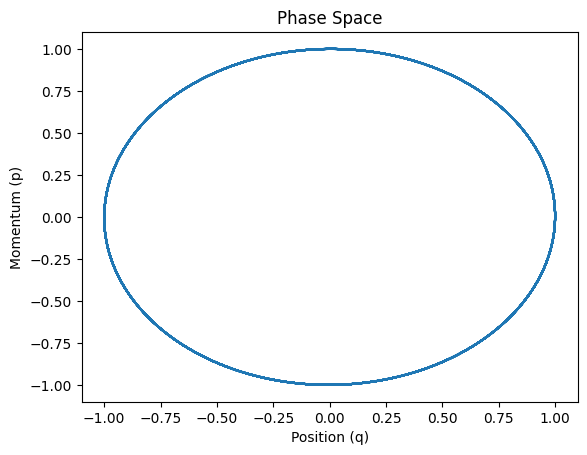
\includegraphics[width=0.5\linewidth]{./Figures/Sympletic/eulerphase.png}
	\caption{Phase space of the harmonic oscillator using the symplectic Euler method with \(\Delta t = 0.01\).}
	\label{fig:eulerphase}
\end{figure}

The Figure~\ref{fig:eulerphase} shows the phase space of the harmonic oscillator using the symplectic Euler method. We can see that the phase space is a closed curve, which is the correct behaviour of the harmonic oscillator.

\begin{figure}[H]
	\centering
	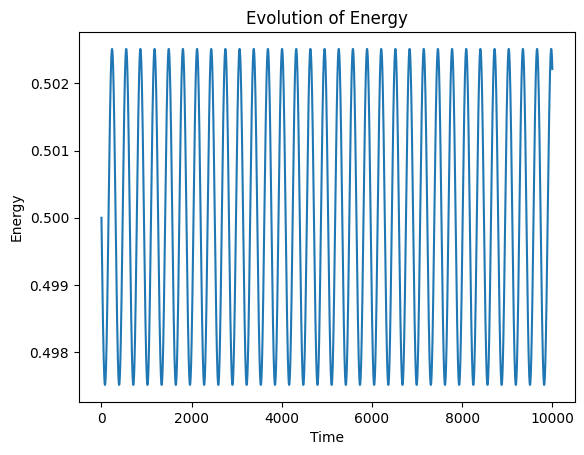
\includegraphics[width=0.5\linewidth]{./Figures/Sympletic/eulerenergy.png}
	\caption{Energy of the harmonic oscillator using the symplectic Euler method with \(\Delta t = 0.01\).}
	\label{fig:eulerenergy}
\end{figure}

The Figure~\ref{fig:eulerenergy} shows the energy of the harmonic oscillator using the symplectic Euler method. We can see that the energy is conserved over time, as we wanted for the Hamiltonian dynamics. Note that is not a straight line but the average of the energy is the same, so we can conclude that the energy is conserved over time.

Now, if we define the next map:
\[
	\Gamma_{\Delta t}^{Euler} = \max_{n \in \mathbb{N}}\{|H_{\Delta t}(p^n, q^n) - H_{\Delta t}(p^0, q^0)|\}
\]

The Figure~\ref*{fig:eulermaxenergy} shows the function \(\Gamma_{\Delta t}^{Euler}\) over \(\frac{1}{\Delta t}\).

\begin{figure}[H]
	\centering
	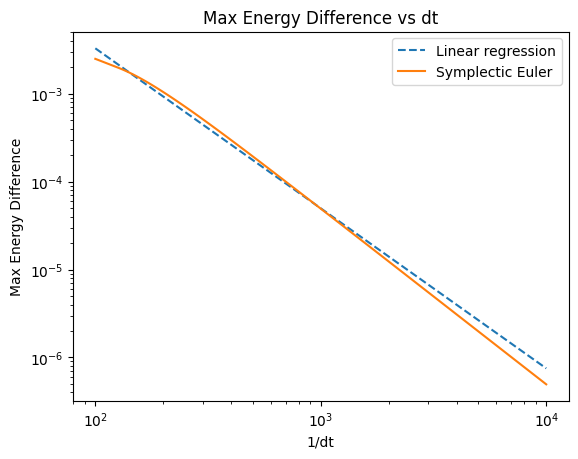
\includegraphics[width=0.5\linewidth]{./Figures/Sympletic/eulermaxenergy.png}
	\caption{Function \(\Gamma_{\Delta t}^{Euler}\) over \(\frac{1}{\Delta t}\)}
	\label{fig:eulermaxenergy}
\end{figure}

To conclude the section, we can see in Figure~\ref*{fig:eulermaxenergy} that the difference decreases as the time step decreases, which is the expected behaviour of any scheme that preserves the symplectic structure of the Hamiltonian dynamics equations. Therefore, we can conclude that the symplectic Euler method is a good method to solve the Hamiltonian dynamics equations.

\subsubsubsection{Linear Stability Analysis of the Sympletic Euler Scheme}
\label{sec:linear_stability_symplectic_euler}

Using the equation \ref{eq:symplecticeuler} and replacing all the termusing the harmonic oscillator problem, one can rewrite the scheme as:

\[
	\begin{pmatrix} p^{n+1} \\ q^{n+1} \end{pmatrix} = A \begin{pmatrix} p^{n} \\ q^{n} \end{pmatrix}
\]

With

\[
	A = \begin{pmatrix}
		1 && -\Delta t k \\
		\frac{\Delta t}{m} && 1
	\end{pmatrix}
\]

Noting \(\xi = \Delta t \sqrt{\frac{k}{m}}\), the eigenvalues are:

\[
	\lambda_1 = 1 + i\xi, \ \ \lambda_2 = 1 - i\xi
\]

In linear stability analysis, a scheme is said to be stable if the eigenvalues of the amplification matrix lie inside the unit circle in the complex plane. This means that their absolute values should be less than or equal to 1 for all possible values of \(\xi\). In this case, their magnitudes are:

\[
	|\lambda_1| = |\lambda_2| = 1 + \xi^2
\]

For stability we require \(|\lambda| \leq 1\). This transalates to the condition:

\[
	1 + \xi^2 \leq 1
\]

Therefore, the sympletic euler scheme isn't stable for any \(\xi\).




\subsubsection{Stormer-Verlet method}
\label{sec:stormer_verlet_method}

The Störmer-Verlet method, often simply referred to as the Verlet method, is a numerical technique used to integrate ordinary differential equations of the form \( \dot{y} = f(y) \). It is particularly popular in molecular dynamics simulations and other problems modeled by Hamiltonian systems. The method can be derived directly from the Taylor series expansion of the solution. The central idea behind the method is to use information from both the current and previous time steps to predict the value at the next time step. 

The Störmer-Verlet method applied to the Hamiltonian equations is as follows (using dHdq and dHdp to denote the partial derivatives of H with respect to q and p, respectively):

\begin{equation}
	\begin{cases}
		p^{n + \frac{1}{2}} = p^n - \frac{\Delta t}{2} \nabla_q V(q^n) \\
		q^{n+1} = q^{n} + \Delta t M^{-1} p^{t+1/2} \\
		p^{n+1} = p^{n+\frac{1}{2}} - \frac{\Delta t}{2} \nabla_q V(q^{n+1})
	\end{cases}
	\label{eq:stormerverlet}
\end{equation}

The numerical flow of this scheme is noted as \(\phi^{Verlet}_t\). In matter of fact, note that:

\[
	\Phi^{Verlet}_{\Delta t} = \phi^2_{\Delta t/2} \circ \phi^1_{\Delta t} \circ \phi^2_{\Delta t}
\]


Therefore, it is easy to prove that, by construction, is a sympletic scheme. So given the problem of the harmonic oscillator using the Störmer-Verlet method, the update equations become:

\begin{equation}
	\begin{cases}
		p^{n + \frac{1}{2}} = p^n - \frac{\Delta t}{2} kq^n \\
		q^{n+1} = q^{n} + \Delta t M^{-1} p^{t+1/2} \\
		p^{n+1} = p^{n+\frac{1}{2}} - \frac{\Delta t}{2} kq^{n+1}
	\end{cases}
	\label{eq:stormerverletharmonic}
\end{equation}

The Figure~\ref{fig:stormerverletphase} shows the phase space of the harmonic oscillator using the Störmer-Verlet method.

\begin{figure}[H]
	\centering
	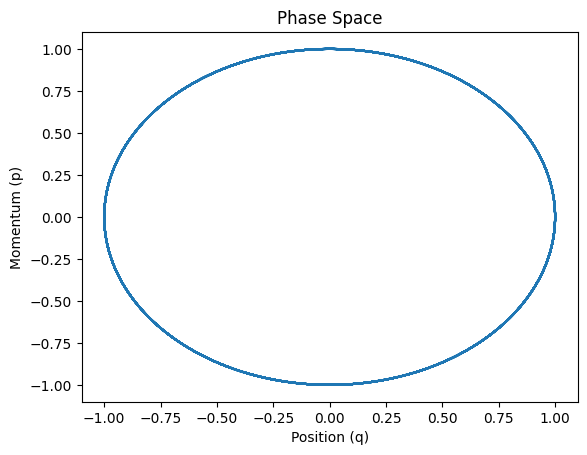
\includegraphics[width=0.5\linewidth]{./Figures/Sympletic/verletphase.png}
	\caption{Phase space of the harmonic oscillator using the Störmer-Verlet method with \(\Delta t = 0.01\).}
	\label{fig:stormerverletphase}
\end{figure}

The Figure~\ref{fig:stormerverletphase} shows the phase space of the harmonic oscillator using the Störmer-Verlet method. We can see that the phase space is a closed curve, which is the correct behaviour of the harmonic oscillator.

\begin{figure}[H]
	\centering
	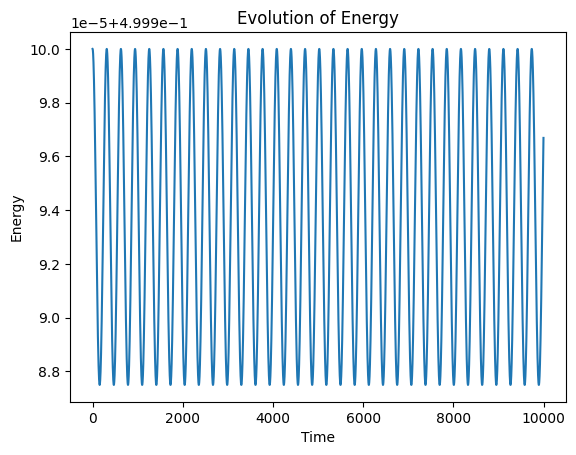
\includegraphics[width=0.5\linewidth]{./Figures/Sympletic/verletenergy.png}
	\caption{Energy of the harmonic oscillator using the Störmer-Verlet method with \(\Delta t = 0.01\).}
	\label{fig:stormerverletenergy}
\end{figure}

The Figure~\ref{fig:stormerverletenergy} shows the energy of the harmonic oscillator using the Störmer-Verlet method. We can see that the energy is conserved over time, as we wanted for the Hamiltonian dynamics. Like the behaviour of the Euler Sympletic method, we can see that in this case, the energy continues to oscillate around the average value, however the scale of this oscillation is much smaller than in the Euler Sympletic method. To see this, we define the following function:

\[
	\Gamma_{\Delta t}^{Verlet} = \max_{n \in \mathbb{N}}\{|H_{\Delta t}(p^n, q^n) - H_{\Delta t}(p^0, q^0)|\}
\]

The Figure~\ref*{fig:stormerverletmaxenergy} shows the function \(\Gamma_{\Delta t}^{Verlet}\) over \(\frac{1}{\Delta t}\).

\begin{figure}[H]
	\centering
	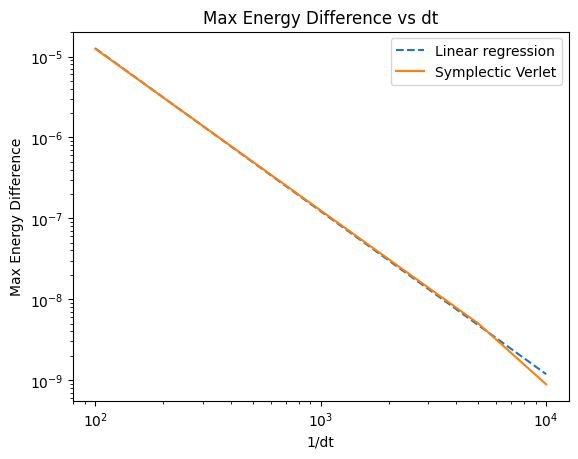
\includegraphics[width=0.5\linewidth]{./Figures/Sympletic/verletmaxenergy.png}
	\caption{Function \(\Gamma_{\Delta t}^{Verlet}\) over \(\frac{1}{\Delta t}.\)}
	\label{fig:stormerverletmaxenergy}
\end{figure}

So now we are prepared to overview the difference between both methods. The Figure~\ref*{fig:comparisonmaxenergy} shows the function \(\Gamma_{\Delta t}^{Euler}\) and \(\Gamma_{\Delta t}^{Verlet}\) over \(\frac{1}{\Delta t}\).

\begin{figure}[H]
	\centering
	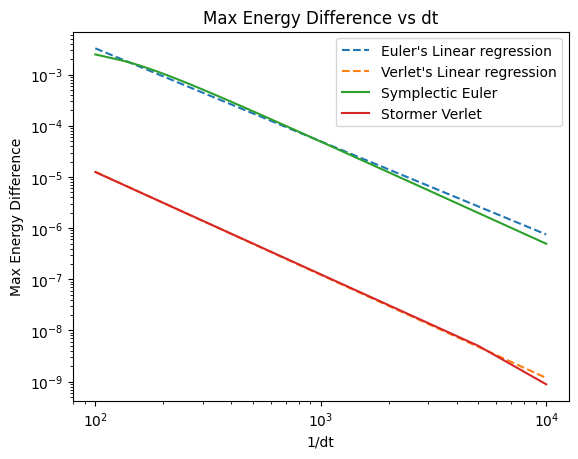
\includegraphics[width=0.5\linewidth]{./Figures/Sympletic/maxenergydifference.png}
	\caption{Function \(\Gamma_{\Delta t}^{Euler}\) and \(\Gamma_{\Delta t}^{Verlet}\) over \(\frac{1}{\Delta t}\)}
	\label{fig:comparisonmaxenergy}
\end{figure}

As we can see, the Störmer-Verlet method is much better than the Euler Sympletic method. Probably, this is a consequence of the fact that the Störmer-Verlet method is a second order method, while the Euler Sympletic method is a first order method. Therefore, we can conclude that the Störmer-Verlet method is a better method to solve the Hamiltonian dynamics equations than the Euler Sympletic method.

\subsubsubsection{Linear Stability Analysis of the Verlet Scheme}
\label{sec:linear_stability_verlet}

Using the equation \ref{eq:stormerverletharmonic} and replacing all the terms by its definition, and considering that \(\omega = \sqrt{\frac{k}{m}}\), we can rewrite the scheme as:

\[
	\begin{pmatrix} p^{n+1} \\ q^{n+1} \end{pmatrix} = A \begin{pmatrix} p^{n} \\ q^{n} \end{pmatrix}
\]

With

\[
	A = \begin{pmatrix}
		1 - \frac{(\omega \Delta t)^2}{2} && \Delta t \\
		-\omega^2 \Delta t (1 - \frac{(\omega \Delta t)^2}{4}) && 1 - \frac{(\omega \Delta t)^2}{2}
	\end{pmatrix}
\]

Noting \(\xi = \frac{(\omega \Delta t)^2}{2}\), the eigenvalues are the solutions of $\lambda$ in:

\[
	(1 - \xi - \lambda)^2 + \xi (2 - \xi) = 0
\]

Therefore, the eigenvalues are:

\[
	\begin{cases}
		\lambda_1 = 1 - \xi + i\sqrt{\xi(2-\xi)} &
		\lambda_2 = 1 - \xi - i\sqrt{\xi(2-\xi)} \ \ if \ \xi(2-\xi) \geq 0 \\

		\lambda_1 = 1 - \xi + \sqrt{\xi(\xi - 2)} &
		\lambda_2 = 1 - \xi - \sqrt{\xi(\xi - 2)} \ \ if \ \xi(2-\xi) \leq 0 \\
	\end{cases}
\]

In linear stability analysis, a scheme is said to be stable if the eigenvalues of the amplification matrix lie inside the unit circle in the complex plane. This means that their absolute values should be less than or equal to 1 for all possible values of \( \xi \). This ensures that errors do not grow unboundedly as we march forward in time.

Given the eigenvalues derived above:

\[
	\lambda_1 = \begin{cases}
		1 - \xi + i\sqrt{\xi(2-\xi)} \ \text{if} \ \xi(2-\xi) \geq 0 \\
		1 - \xi + \sqrt{\xi(\xi - 2)} \ \text{if} \ \xi(2-\xi) \leq 0 \\
	\end{cases}
\]

\[
	\lambda_2 = \begin{cases}
		1 - \xi - i\sqrt{\xi(2-\xi)} \ \text{if} \ \xi(2-\xi) \geq 0 \\
		1 - \xi - \sqrt{\xi(\xi - 2)} \ \text{if} \ \xi(2-\xi) \leq 0 \\
	\end{cases}
\]

The eigenvalues are complex conjugates. Their magnitudes are:

\[
	|\lambda_1| = |\lambda_2| = \sqrt{(1 - \xi)^2 + \xi(2-\xi)} 
\]

For stability, we require \( |\lambda_1| \leq 1 \). This translates to the condition:

\[
	(1 - \xi)^2 + \xi(2-\xi) \leq 1
\]

This inequality leads to a tautology so it is always stable. This is consistent with the observed property of the Störmer-Verlet scheme which conserves the energy over time and doesn't let errors gro unboundedly. This, in combination with its second-order accuracy, makes it preferable over the Euler sympletic method for problems modeled by Hamiltonian systems.

\subsubsection{Backward Error Analysis}
\label{sec:backward_error_analysis}

In this section, we will introduce the backward error analysis. The backward error analysis is a technique to analyze the error of a numerical method. We can define the idea of this technique as: For a given problem \(P(x)\), an exact input \(x\) and an approximate solution \(\hat{x}\), we can define the backward error as the smallest perturbation \(\Delta x\) such that \(P(x + \Delta x) = \hat{x}\). Therefore the formal definitions, extracted with little modifications from \cite{fraysse2018hdr}, is:

\begin{definition}[Backward error]
	Let \(\hat{x}\) be an approximate solution to the equation \(P(d) = x\). Then the backward error of \(\hat{x}\) is defined by:
	\[
		\eta = \min \{ \epsilon : P(x + \Delta x) = \hat{x}, ||\Delta x|| \leq \epsilon \}
	\]
\end{definition}

The following Figure~\ref{fig:backwarderror} extracted from \cite{higham2020backwarderror} illustrated the idea of the backward error analysis.

\begin{figure}[H]
	\centering
	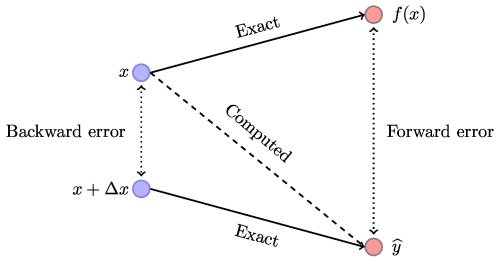
\includegraphics[width=0.5\linewidth]{./Figures/Sympletic/graphic.jpg}
	\caption{Backward error analysis.}
	\label{fig:backwarderror}
\end{figure}








\subsection{Solar System Simulation}
\label{sec:solar_system_simulation}

In this section, we'll harness the power of Hamiltonian dynamics to craft a simulation of the solar system. We'll adopt the Stormer-Verlet scheme, renowned for its energy-conserving properties, as our primary numerical method.

First of all, let's do a brief introduction to the problem we want to solve. We can see the solar system as a set of \(N\) bodies, each of them with a mass \(m_i\) a position \(q_i\) and a velocity \(v_i\). The position and velocity are vectors in \(\mathbb{R}^2\). The gravitational force between two bodies is given by:

\subsubsection{Modeling the Solar System: Gravitational Dynamics}
\label{sec:modeling_solar_system}

The motion of celestial bodies in the solar system, primarily planets, moons, and the Sun, can be described by Newton's law of universal gravitation. For \(N\) bodies, the gravitational force exerted on the \(i^{th}\) body due to the \(j^{th}\) body is given by:

\[
\mathbf{F}_{ij} = -\frac{G m_i m_j (\mathbf{q}_i - \mathbf{q}_j)}{|\mathbf{q}_j - \mathbf{q}_i|^3}
\]

where \(G\) is the gravitational constant, approximately \(6.67430 \times 10^{-11} \ \text{Nm}^2/\text{kg}^2\), \(\mathbf{q}_i\) and \(\mathbf{q}_j\) are the position vectors of the \(i^{th}\) and \(j^{th}\) bodies respectively and \(m_i\) and \(m_j\) are the masses of the \(i^{th}\) and \(j^{th}\) bodies respectively. Therefore, the total gravitational force acting on the \(i^{th}\) body due to all other bodies is:

\[
	\mathbf{F}_i = \sum_{j=1, j\neq i}^{N} \mathbf{F}_{ij}
\]

To use Hamiltonian mechanics and the Störmer-Verlet scheme, we can represent the system in terms of its Hamiltonian, which is the sum of its kinetic and potential energies. For the \(i^{th}\) body:

1. Kinetic Energy, \(T_i\):

\[
	T_i = \frac{1}{2} m_i \mathbf{v}_i \cdot \mathbf{v}_i
\]

where \(\mathbf{v}_i\) is the velocity of the \(i^{th}\) body.

2. Potential Energy, \(U_{ij}\), due to the interaction between the \(i^{th}\) and \(j^{th}\) bodies:

\[
	U_{ij} = -\frac{G m_i m_j}{|\mathbf{q}_j - \mathbf{q}_i|}
\]

The total Hamiltonian \(H\) for the system is the sum of the kinetic and potential energies for all body pairs:

\[
	H = \sum_{i=1}^{N} T_i + \frac{1}{2} \sum_{i=1}^{N} \sum_{j=1, j\neq i}^{N} U_{ij}
\]

This Hamiltonian can be used to derive the equations of motion using Hamilton's equations, which can then be solved using the Störmer-Verlet scheme.

In the next section, we'll dive deeper into the implementation details, but this sets up the mathematical foundation for our solar system simulation based on gravitational interactions.

\subsubsection{Störmer-Verlet Scheme for Gravitational Dynamics}
\label{sec:stormer_verlet_scheme_gravitational_dynamics}

Now that we have the Hamiltonian for the system, we can derive use it inside the Störmer-Verlet scheme to derive the equations of motion. The Störmer-Verlet scheme for the \(i^{th}\) body is:

\[
	\begin{cases}
		\mathbf{p}_i^{n + \frac{1}{2}} = \mathbf{p}_i^n - \frac{\Delta t}{2} \nabla_{\mathbf{q}_i} U(\mathbf{q}^n_i) \\
		\mathbf{q}_i^{n+1} = \mathbf{q}_i^{n} + \Delta t M^{-1} \mathbf{p}_i^{n+1/2} \\
		\mathbf{p}_i^{n+1} = \mathbf{p}_i^{n+\frac{1}{2}} - \frac{\Delta t}{2} \nabla_{\mathbf{q}_i} U(\mathbf{q}^{n+1}_i)
	\end{cases}
\]

where \(U(\mathbf{q}_i)\) is the potential energy of the \(i^{th}\) body due to all other bodies. The total potential energy of the system is the sum of the potential energies of all body pairs:

\[
	U = \frac{1}{2} \sum_{i=1}^{N} \sum_{j=1, j\neq i}^{N} U_{ij}
\]

where \(U_{ij}\) is the potential energy of the \(i^{th}\) body due to the \(j^{th}\) body. Therefore, the gradient of the potential energy of the \(i^{th}\) body is:

\[
	\nabla_{\mathbf{q}_i} U(\mathbf{q}_i) = 
		\nabla_{\mathbf{q}_i} U(\mathbf{q}_i) = \sum_{j=1, j\neq i}^{N} \nabla_{\mathbf{q}_i} U_{ij}(\mathbf{q}_i, \mathbf{q}_j)
\]
		
Given that:
		
\[
	U_{ij} = -\frac{G m_i m_j}{|\mathbf{q}_j - \mathbf{q}_i|}
\]
		
We can compute the gradient of \(U_{ij}\) with respect to \(\mathbf{q}_i\). Firstly, we can express the distance \(|\mathbf{q}_j - \mathbf{q}_i|\) as \(r_{ij}\):

\[ 
	r_{ij} = |\mathbf{q}_j - \mathbf{q}_i| 
\]

Thus, the potential energy becomes:

\[ 
	U_{ij} = -\frac{G m_i m_j}{r_{ij}} 
\]

To find the gradient of \(U_{ij}\) with respect to \(\mathbf{q}_i\), we need to differentiate with respect to \(\mathbf{q}_i\):

\[ 
	\nabla_{\mathbf{q}_i} U_{ij} = \frac{\partial U_{ij}}{\partial r_{ij}} \frac{\partial r_{ij}}{\partial \mathbf{q}_i} 
\]

First, differentiate \(U_{ij}\) with respect to \(r_{ij}\):

\[ 
	\frac{\partial U_{ij}}{\partial r_{ij}} = G m_i m_j \frac{1}{{r_{ij}}^2} 
\]

Next, differentiate \(r_{ij}\) with respect to \(\mathbf{q}_i\):

\[ 
	r_{ij} = \sqrt{(\mathbf{q}_j - \mathbf{q}_i) \cdot (\mathbf{q}_j - \mathbf{q}_i)} 
\]

\[ 
	\frac{\partial r_{ij}}{\partial \mathbf{q}_i} = \frac{\mathbf{q}_j - \mathbf{q}_i}{{r_{ij}}} 
\]

Putting it all together:

\[ 
	\nabla_{\mathbf{q}_i} U_{ij} = G m_i m_j \frac{1}{{r_{ij}}^2} \frac{\mathbf{q}_i - \mathbf{q}_j}{{r_{ij}}} = G m_i m_j \frac{\mathbf{q}_i - \mathbf{q}_j}{{r_{ij}}^3} 
\]

Thus, the gradient of the potential energy \(U_{ij}\) with respect to \(\mathbf{q}_i\) is:
		
\[
	\nabla_{\mathbf{q}_i} U_{ij} = - G m_i m_j \frac{\mathbf{q}_i - \mathbf{q}_j}{|\mathbf{q}_j - \mathbf{q}_i|^3}
\]
		
Now, plugging this back into the equation for the gradient of the total potential energy with respect to \(\mathbf{q}_i\):
		
\[
	\nabla_{\mathbf{q}_i} U(\mathbf{q}_i) = \sum_{j=1, j\neq i}^{N} - G m_i m_j \frac{\mathbf{q}_i - \mathbf{q}_j}{|\mathbf{q}_j - \mathbf{q}_i|^3}
\]
		
This is the gradient of the potential energy with respect to the position of the \(i^{th}\) body, taking into account all the interactions with other bodies in the system. Before executing the Störmer-Verlet scheme, let's show the potential energy of the system. The Figure~\ref{fig:potentialenergy} shows the potential energy of the system.

\begin{figure}[H]
	\centering
	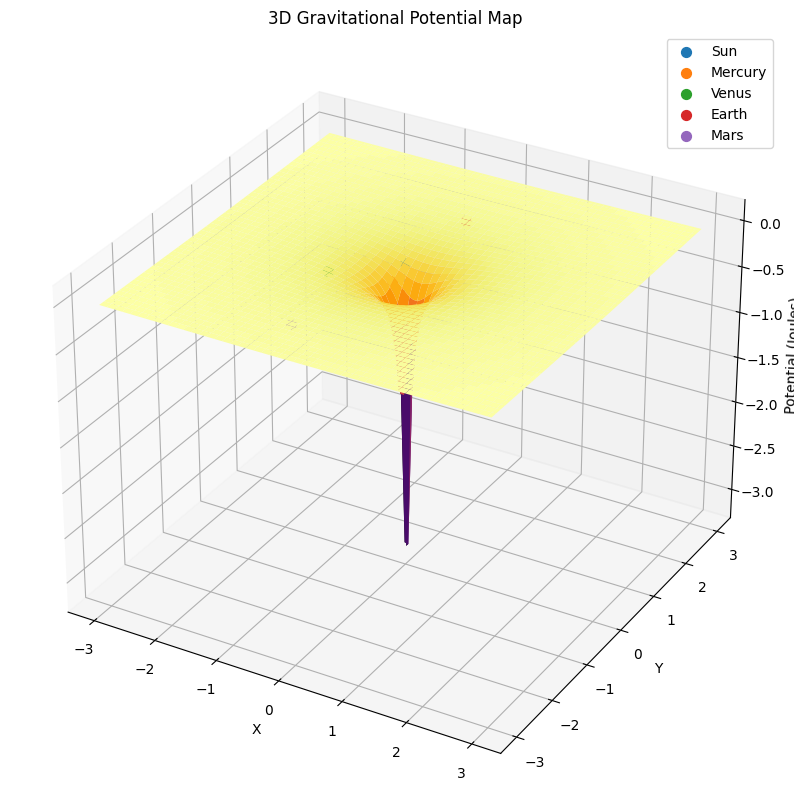
\includegraphics[width=0.5\linewidth]{./Figures/SolarSystem/gravitationalpotential.png}
	\caption{Potential energy of the part of the solar system.}
	\label{fig:potentialenergy}
\end{figure}
As we could have expected, the Sun has, by far, the most negative potential energy, since it is the body with the highest mass. Also we can observe that the potential energy is negative, which is the expected behaviour of the gravitational potential energy. 

\subsubsection{Implementation of the Solar System Simulation}
\label{sec:implementation_solar_system}

First of all, we need to define the parameters of the simulation. The Table~\ref{table:parameters} shows the parameters of the simulation.

\begin{table}[H]
	\centering
	\renewcommand{\arraystretch}{1.2} % Adjusts the row height
	\begin{tabular}{>{\bfseries}l >{\raggedleft}p{3cm} >{\raggedleft\arraybackslash}p{3cm} >{\raggedleft\arraybackslash}p{3cm}}
	\toprule
	\textbf{Celestial Body} & \textbf{Mass (Relative to Sun)} & \textbf{Position (AU)} & \textbf{Mean velocity (AU/Year)} \\
	\midrule
	Sun       & 1.0000    & 0.000 & 0.00 \\
	Mercury   & 1.6505e-7 & 0.390 & 9.99 \\
	Venus     & 2.4335e-6 & 0.720 & 7.38 \\
	Earth     & 2.9860e-6 & 1.000 & 6.28 \\
	Mars      & 3.2085e-7 & 1.520 & 5.08 \\
	Jupiter   & 9.4950e-4 & 5.187 & 2.76 \\
	\bottomrule
	\end{tabular}
	\caption{Data of Celestial Bodies in the Solar System}
	\label{table:parameters}
\end{table}

Therefore, the units that we have used are:

\begin{itemize}
	\item Mass: \(M_{\odot}\) (Solar Mass)
	\item Distance: AU (Astronomical Unit)
	\item Time: Earth year
\end{itemize}

This is because we want to do a simulation of the solar system inside a machine that uses discrete numbers, therefore if we use the SI units, we could get some troubles with the precision of the machine, while if we use the units that we have used, we get numbers that are not too big or too small, so we can get a good precision. Also, using this numbers we get that the gravitational constant is:

\[
	G = 4 \pi^2 \ \frac{\text{AU}^3}{\text{year}^2 \ M_{\odot}}
\]

Note that we have used the real masses of the planets and the Sun, and the real distance between them. Therefore, we can see that the simulation is very similar to the real solar system. All of these parameters can be found on the NASA website \cite{nssdc2022planetaryfactsheet}. Now we are prepared to implement the simulation. 

For illustrative purposes, we'll simulate the orbits of the Sun, Mercury, Venus, Earth and Mars. The Figure~\ref{fig:solarsystem} shows the orbits of the planets of the solar system during 365 days and with a time step of 1 day.

\begin{figure}[H]
	\centering
	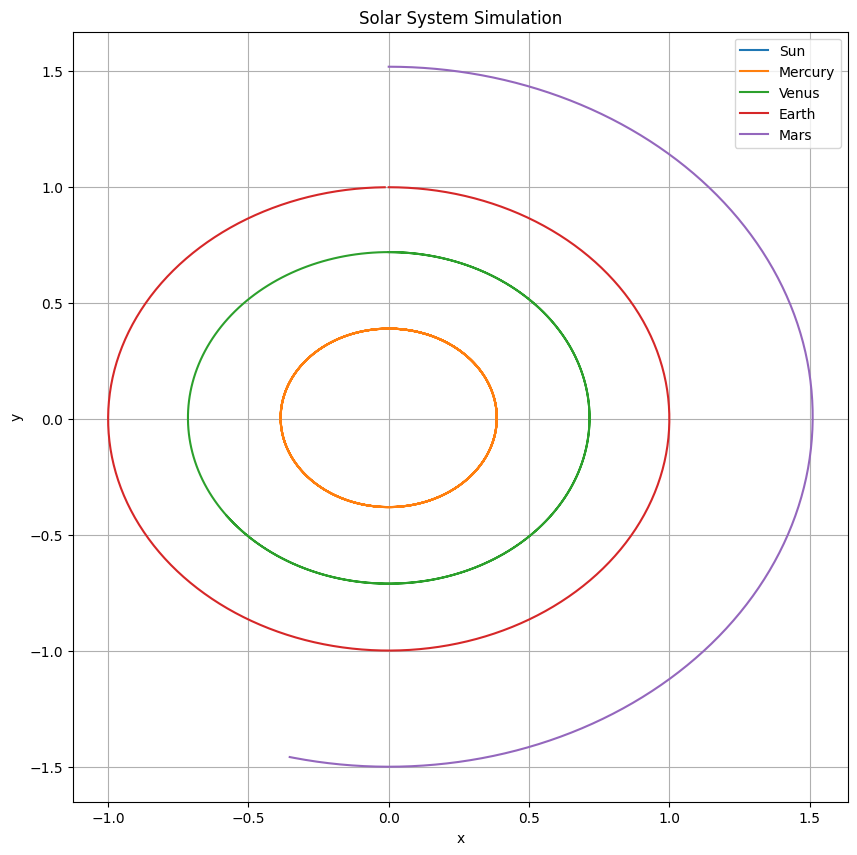
\includegraphics[width=0.5\linewidth]{./Figures/SolarSystem/orbits.png}
	\caption{Simulation of the orbits of part of the planets of the solar system using the Störmer-Verlet scheme for \(\Delta t = 1\) day and \(T = 365\) days.}
	\label{fig:solarsystem}
\end{figure}

We can see that the orbits are closed curves, which is the expected behaviour of the planets of the solar system. Also, we can see that the orbits are not perfect circles, which is also the expected behaviour of the planets of the solar system. 

Now let's see the energy of the system. The Figure~\ref{fig:solarsystemenergy1} shows the energy of the system for the same simulation.

\begin{figure}[H]
	\centering
	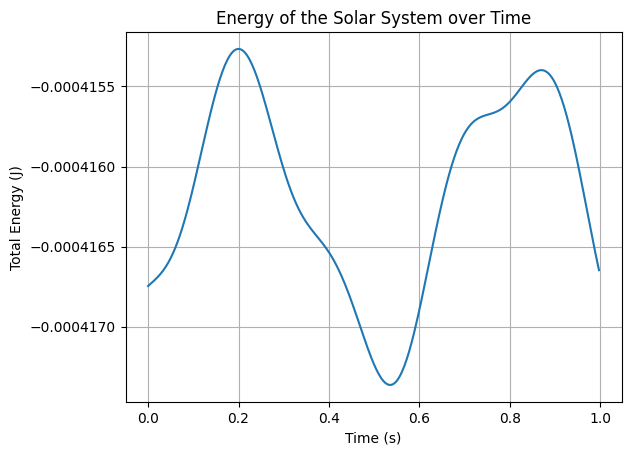
\includegraphics[width=0.5\linewidth]{./Figures/SolarSystem/energy1.png}
	\caption{Energy of the simulation of part of the planets of the solar system using the Störmer-Verlet scheme for \(\Delta t = 1\) day and \(T = 365\) days.}
	\label{fig:solarsystemenergy1}
\end{figure}

We can see that the energy is conserved over time, as we wanted for the Hamiltonian dynamics. Note that is not a straight line but the average of the energy is the same and we can see a slight of oscillations that may be repeated in the future if the simulation is done for more time. So, let's do the simulation for 20 years. The Figure~\ref{fig:solarsystemenergy2} shows the energy of the system for the same simulation.

\begin{figure}[H]
	\centering
	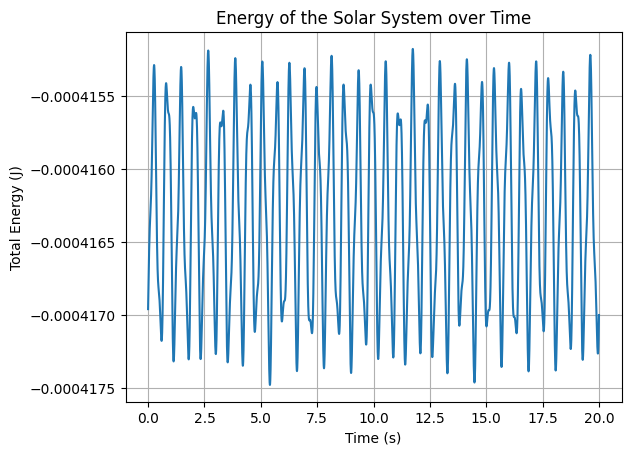
\includegraphics[width=0.5\linewidth]{./Figures/SolarSystem/energy2.png}
	\caption{Energy of the simulation of part of the planets of the solar system using the Störmer-Verlet scheme for \(\Delta t = 1\) day and \(T = 20\) years.}
	\label{fig:solarsystemenergy2}
\end{figure}

As predicted, we can observe that the energy is preserved.

Now that we have the system created and we have seen that the energy is preserved, we can do some experiments. 

\subsubsubsection{Experiment 1: Expanding to the N-Body Problem}
\label{sec:expanding_n_body_problem}

In our initial simulation, as detailed in the referenced table, we included data for Jupiter but did not incorporate it into the actual simulation. This was primarily due to Jupiter's significant distance from the inner planets, which could potentially complicate the visual clarity of our model. However, given Jupiter's substantial mass – the largest among the planets – its inclusion is crucial for a more comprehensive understanding of the solar system's dynamics. This necessitates an expansion of our model to an N-body problem, allowing for the gravitational influence of not just the Sun but also the other planets to be accounted for.

To explore this, we have extended our simulation to include Jupiter, aiming to observe its impact on the orbital paths of the other planets. The updated Figure~\ref{fig:solarsystemjupiter} illustrates the orbits of the solar system's planets over a period of 20 years with a daily time step, now incorporating Jupiter. This addition provides a more realistic and complex representation of the gravitational interplay within our solar system.

\begin{figure}[H]
	\centering
	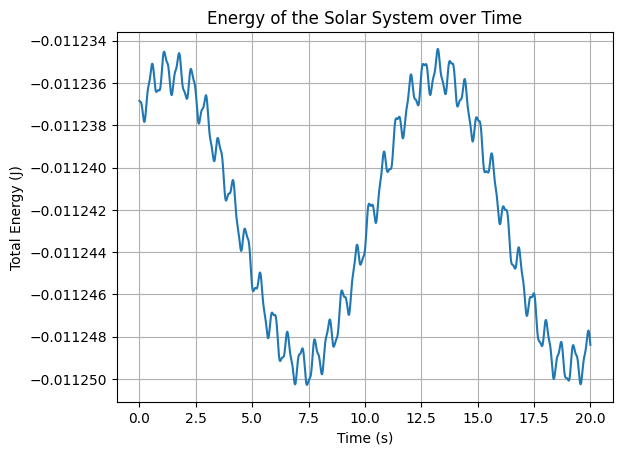
\includegraphics[width=0.5\linewidth]{./Figures/SolarSystem/orbitsjupiter.png}
	\caption{Simulation of the orbits of the planets of the solar system using the Störmer-Verlet scheme for \(\Delta t = 1\) day and \(T = 20\) years, now including Jupiter.}
	\label{fig:solarsystemjupiter}
\end{figure}


\subsubsubsection{Experiment 2: Using Symplectic Euler Method}
\label{sec:using_symplectic_euler_method}

We alredy know that the Störmer-Verlet method performs better than the Euler Symplectic method, but let's see how the solar system behaves using the Euler Sympletic method. The Figure~\ref{fig:solarsystemeuler} shows the orbits of the planets of the solar system using the Euler Symplectic method for \(\Delta t = 1\) day and \(T = 20\) years.

\begin{figure}[H]
	\centering
	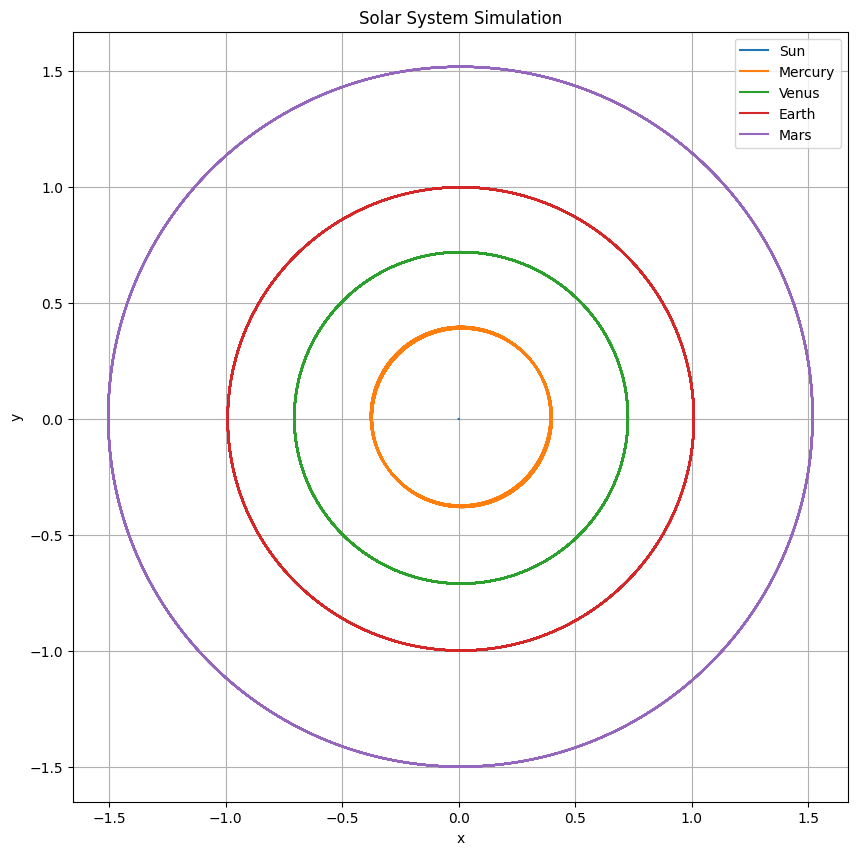
\includegraphics[width=0.5\linewidth]{./Figures/SolarSystem/orbits_euler.png}
	\caption{Simulation of the orbits of the planets of the solar system using the Euler Sympletic method for \(\Delta t = 1\) day and \(T = 20\) years.}
	\label{fig:solarsystemeuler}
\end{figure}

Also we can plot the energy of the system. The Figure~\ref{fig:solarsystemenergyeuler} shows the energy of the system for the same simulation.

\begin{figure}[H]
	\centering
	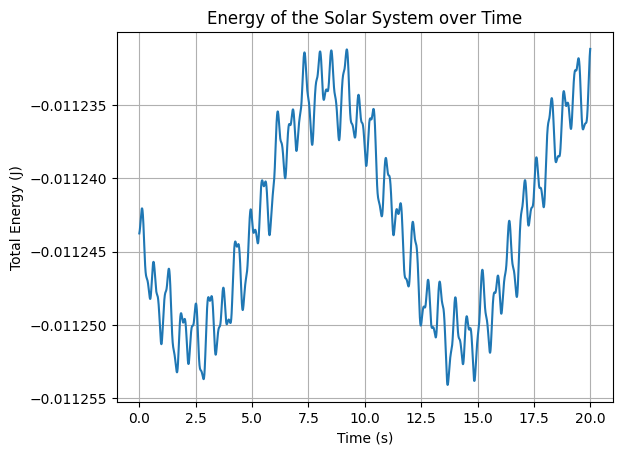
\includegraphics[width=0.5\linewidth]{./Figures/SolarSystem/energy_euler.png}
	\caption{Energy of the simulation of the orbits of the planets of the solar system using the Euler Sympletic method for \(\Delta t = 1\) day and \(T = 20\) years.}
	\label{fig:solarsystemenergyeuler}
\end{figure}

Comparing it to the results obtained using the Störmer-Verlet method, again we can see that the first one is better in the following table:

\begin{table}[H]
	\centering
	\renewcommand{\arraystretch}{1.2} % Adjusts the row height
	\begin{tabular}{>{\bfseries}l >{\raggedleft}p{4cm} >{\raggedleft\arraybackslash}p{4cm} >{\raggedleft\arraybackslash}p{3cm}}
	\toprule
	\textbf{Method} & $\max{H(x)} - \min{H(x)}$  & $\max{|H(X) - \mathbb{E}(H(X))|}$\\
	\midrule
	Symplectic Euler & 7.29e-6 & 3.64e-6  \\
	Störmer-Verlet   & 2.32e-6 & 1.16e-6 \\
	\bottomrule
	\end{tabular}
	\caption{Data of Celestial Bodies in the Solar System}
	\label{table:comparison}
\end{table}

Therefore, in this problem we can conclude that the Störmer-Verlet method is $3.14$ times better in terms of conservation of the Energy than the Euler Sympletic method.

\bibliographystyle{plain}
\bibliography{mybib.bib}
\end{document}
